%\documentclass[10pt, red, draft]{beamer}
\documentclass[10pt, red]{beamer}

\mode<presentation>

%\usetheme{Singapore}
%\usecolortheme{dove}         %%%%%   <<<<<------- descomentar para colcoar tema cinza serio!
%\usecolortheme{orchid}

\usetheme{Warsaw}
\usecolortheme{lily}
\useinnertheme{rectangles}
\useoutertheme[subsection=false]{smoothbars}

\usepackage[brazil]{babel}     
\usepackage[utf8]{inputenc}
\usepackage[T1]{fontenc}
\usepackage{color, colortbl}
%\usepackage[utf8]{inputenc}
%\usepackage[portuges]{babel}

%\usepackage{amsmath}
\usepackage{subfigure}
\usepackage{algorithm}
\usepackage[noend]{algpseudocode}
\usepackage{multirow}

\usepackage{booktabs}

\usepackage{chngpage}
\usepackage{color, colortbl}
\usepackage{fancybox}
\usepackage{graphicx,url}  % for using figures and url format
\usepackage{graphics}
\usepackage{epsfig}

%\usepackage{booktabs,colortbl,tabularx}
\usepackage{booktabs}
\usepackage{textcomp}

%\usepackage[T1]{fontenc}   % avoids warnings such as "LaTeX Font Warning: Font shape 'OMS/cmtt/m/n' undefined"
%\usepackage[caption=false,font=footnotesize]{subfig}
%\usepackage{times}
%\usepackage{latexsym}
%\usepackage{amssymb}
%\usepackage{rotating}
%\usepackage{amssymb}
%\usepackage{ae}
%\usepackage{fix-cm}
\newcommand{\triangOK}{\textcolor[rgb]{00,0.45,0.10}{$\blacktriangle$}}
\newcommand{\triangBAD}{\textcolor[rgb]{0.7,00,00}{$\blacktriangledown$}}
\newcommand{\ball}{\textcolor[rgb]{0.7,0.70,0.0}{$\bullet$}}

\usepackage{tikz}
\usetikzlibrary{shapes,arrows}

\definecolor{LightCyan}{rgb}{0.90,0.9,1}
\definecolor{LightCyan2}{rgb}{0.70,0.9,1}

%\newcommand{\cred}{\textcolor[rgb]{1,0,0}{ }}
\newcommand*\cred[1]{\textcolor[rgb]{1,0,0}{#1}}   % cred -> color red! =P


\def\Tiny{\fontsize{5.3pt}{5.5pt}\selectfont}
\def\SuperTiny{\fontsize{2.3pt}{3.5pt}\selectfont}
\newcommand{\UltraTiny}{\fontsize{0.2pt}{1.0pt}\selectfont}

\title{Credibilidade de exemplos em classificação automática.}
\author[João Rafael de Moura Palotti]{Jo\~{a}o Rafael de Moura Palotti \\ \and Gisele L. Pappa}
%\advisor{Michael}
%\principaladviser{Gisele L. Pappa}
%\adviser{Gisele L. Pappa}
\date{Setembro, 2011}
\institute[DCC - UFMG]
{
%\subfigure[][a]{
%       
\includegraphics[width=0.35\textwidth]{Figures/logoufmg.eps}
%}
%\subfigure[][b]{
%    \includegraphics[width=0.35\textwidth]{Figures/dcclogo.eps}
%}

\includegraphics[width=0.3\textwidth]{Figures/logoufmg.eps}\\%remove this line if no logo
DCC - Departamento de Ciência da Computação\\UFMG - Universidade Federal de Minas Gerais
}

\begin{document}

\frame{\titlepage}

%\section[Outline]{}
%\frame{
%\frametitle{Outline}
%    \tableofcontents
%}

\AtBeginSection[]
{
 \begin{frame}<beamer>{Índice}
    \tableofcontents[currentsection]
     \end{frame}
}


\section{Introdução}

\subsection{Classificação}
\frame{
    \frametitle{Classificação}
    \begin{itemize}

%        \item Partindo da premissa que dois exemplos estão em uma mesma classe se eles possuem um valor semântico próximo, \textbf{classificar} consiste em estipular a qual classe, dentre as disponíveis, um certo exemplo pertence.
   
%        \pause
        \item Em termos práticos:
            \begin{enumerate}
                \item Observamos os indícios do que já conhecemos a fim de criar um \textbf{modelo de classificação}.
                \item Usamos o modelo para prever qual será a classe dos exemplos que não conhecemos ainda.
            \end{enumerate}
    \end{itemize}


\begin{figure}
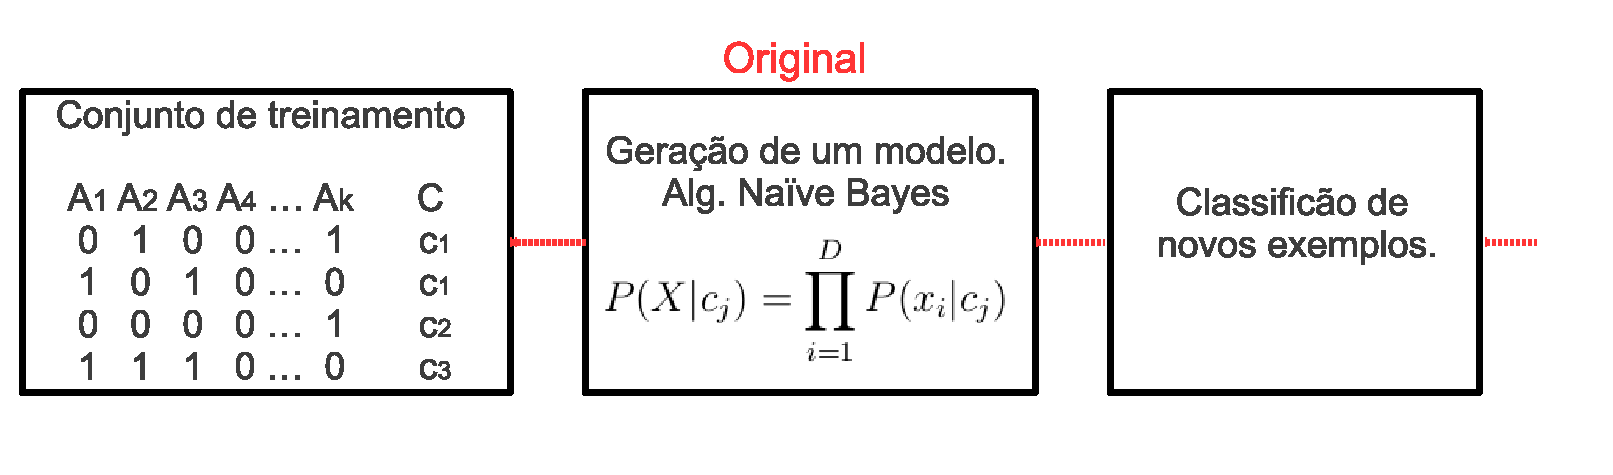
\includegraphics[width=0.9\textwidth]{Figures/workflow-basico.eps}    
\vspace{-0.2cm}
\caption{Esquema tradicional de classificação usando \textit{Naïve Bayes}.}
\end{figure}

}

%\subsection{Exemplos}
%\frame{
%
%    \frametitle{Exemplos - classificação simples}
%    
%    \begin{itemize}
%        
%        \item Terremotos na escala Richter: classificação ``simples'', mas com efeitos complexos.
%        \item Dado um conjunto de variáveis medidas (pressão, amplitude sísmica, vento) de vários terremotos que já ocorreram, o algoritmo de classificação deverá aprender qual a relação existente entre as variáveis e as classes (magnitude) de cada terremoto.
%    \end{itemize}
%
%    \begin{table}[b]
%      \centering
%        \caption{Principais parâmetros utilizados no \textsc{PG}.}
%        \label{tab::parametros}
%
%\pause
%
%\begin{adjustwidth}{-0.75cm}{-0.75cm}% adjust the L and R margins by 1 inch
%\begin{tabular}{cccc|c}
%\toprule 
%\multicolumn{4}{c|}{\textbf{Atributos}} & \multirow{2}{*}{\textbf{Classe}}\tabularnewline
%\cline{1-4} 
%\textbf{Pressão(atm)} & \textbf{Ampl. Sísmica} & \textbf{Vel. Vento(km/h)}& \textbf{Temp.(C)} & \tabularnewline
%\midrule
%1 & 10 & 2.2 & 26.0 & 1\tabularnewline
%0.8 & 1000 & 0.0 & 15.5 & 3\tabularnewline
%1.7 & 100 & 0.4 & 31.2 & 2\tabularnewline
%0.4 & 10000000 & 6.0 & 7.4 & 7\tabularnewline
%\bottomrule
%\end{tabular}
%\end{adjustwidth}
%\end{table}
%
%}
%
%\frame{
%
%
%    \frametitle{Exemplos - classificação muito complexa}
%
%    \begin{itemize}
%        
%        \item A \textit{Standard and Poors} recentemente classificou a nota de risco de investimentos nos EUA como \textsc{AA}.
%        \item A nota atual do Brasil é \textsc{BBB}.
%        \item Baseado em uma série de complexas variáveis que incluem relacionamentos entre os países, diversos fatores econômicos, fatores temporais, etc.
%
%    \end{itemize}
%
%\pause
%\begin{table}[b]
%      \centering
%%        \caption{Principais parâmetros utilizados no \textsc{PG}.}
%        \label{tab::parametros}
%\begin{tabular}{cccc|c}
%\toprule 
%\multicolumn{4}{c|}{\textbf{Atributos}} & \multirow{2}{*}{\textbf{Nota}}\tabularnewline
%\cline{1-4} 
%\textbf{País} & \textbf{PIB/capita} & \textbf{Inflação} & ... & \tabularnewline
%\midrule
%Brasil & \$10,800 & 5\% & ... & \textsc{BBB}-\tabularnewline
%EUA & \$47,200 & 1.6\% & ... & \textsc{AA}+\tabularnewline
%Itália & \$30,500  & 1.6\% & ... & \textsc{A}\tabularnewline
%Liechtenstein & \$141,100  & 0.7\% & ... & \textsc{AAA}\tabularnewline
%\hline 
%\end{tabular}
%\end{table}
%}
%

\frame{

    \frametitle{Exemplos - Classificação textual}
    
    \begin{itemize}
        \item Livros, documentos, artigos, emails, entre outros. 
        \item Dado um conjunto de caracteres que formam um texto (tipicamente palavras, pontuação, etc), a qual classe(s) esse texto pertence?
    \end{itemize}

\pause

\begin{columns}

\column{0.7\textwidth}

\begin{table}[b]
\begin{adjustwidth}{0.1cm}{-0.4cm}% adjust the L and R margins by 1 inch
\small
\begin{tabular}{cccc|c}
\toprule 
\multicolumn{4}{c|}{Atributos} & \multirow{2}{*}{Classe}\tabularnewline
\cline{1-4} 
Livro & Abacate & ... & Zurzir & \tabularnewline
\midrule
Receita Minuto & 1 & ... & 0 & Culinária\tabularnewline
Receita Reunidas & 0 & ... & 0 & Culinária\tabularnewline
Receitas Brasil & 1 & ... & 0 & Culinária\tabularnewline
Sagarana & 0 & ... & 1 & Romance\tabularnewline
G. Sertão: Veredas& 0 & ... & 0 & Romance\tabularnewline
\bottomrule
\end{tabular}
\end{adjustwidth}
\end{table}

\column{0.5\textwidth}
\hspace{0.3cm}
\begin{figure}
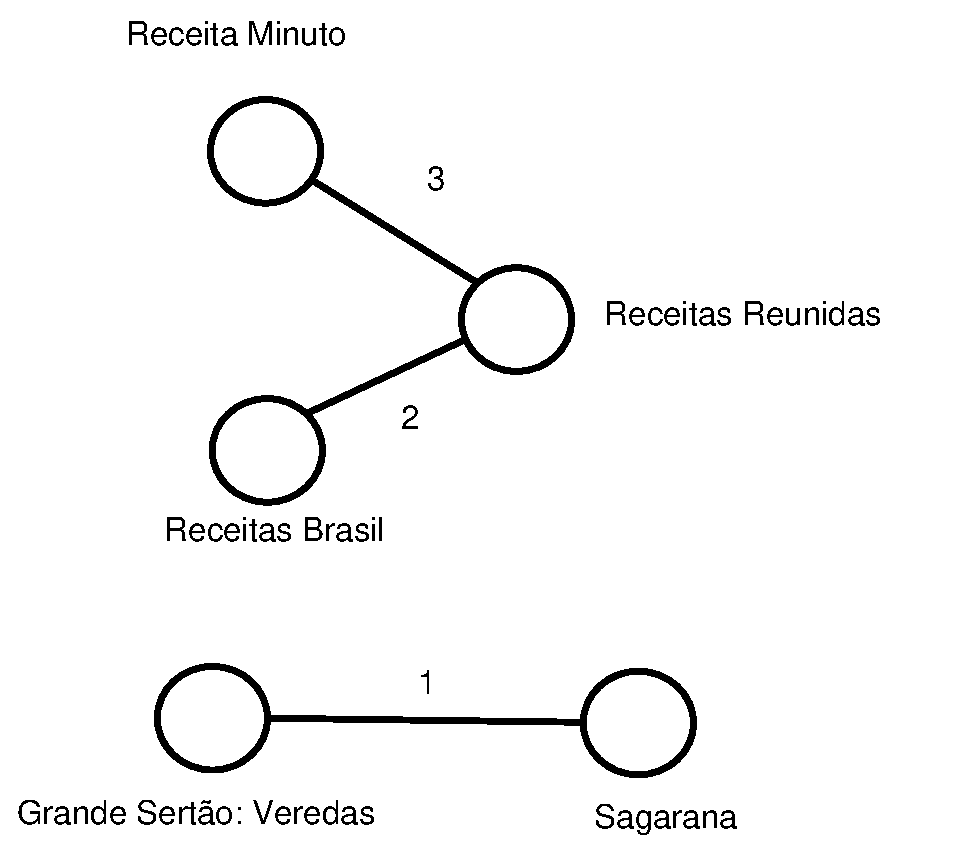
\includegraphics[width=0.9\textwidth]{Figures/grafo-livros.eps}
\end{figure}

\end{columns}

}

\frame{
    \frametitle{Exemplo com Credibilidade}

    \begin{center}
    \begin{itemize}
        \item Diagnóstico médico automático: Dado que tenho uma dor X, qual será o nome da minha enfermidade?

        \pause
            \begin{itemize}
                \item Alguém no \textit{Yahoo} Respostas diz que é A.
                \vskip0.5cm
        
        \pause
                \item Dr. Nick Riviera, seu vizinho, diz que a doença é A.
                \vskip0.5cm

        \pause
                \item Reportagem na revista \textit{Science} diz que é B.
                \vskip0.5cm
            \end{itemize}

    \pause
        \item Como decidir?
    \end{itemize}
    \end{center} 
    
    \bigskip
    \bigskip
    \bigskip

    \UltraTiny
        \begin{center}
        \line(1,0){250}
        \end{center}
    \vspace{-0.5cm}
    O Ministério da Saúde adverte: em qualquer suspeita de uma doença desconhecida (ou mesmo conhecida), um médico deverá ser consultado.
}

\frame{
    \frametitle{Esquema gráfico (baseado no \textsc{KNN})}

\begin{figure}
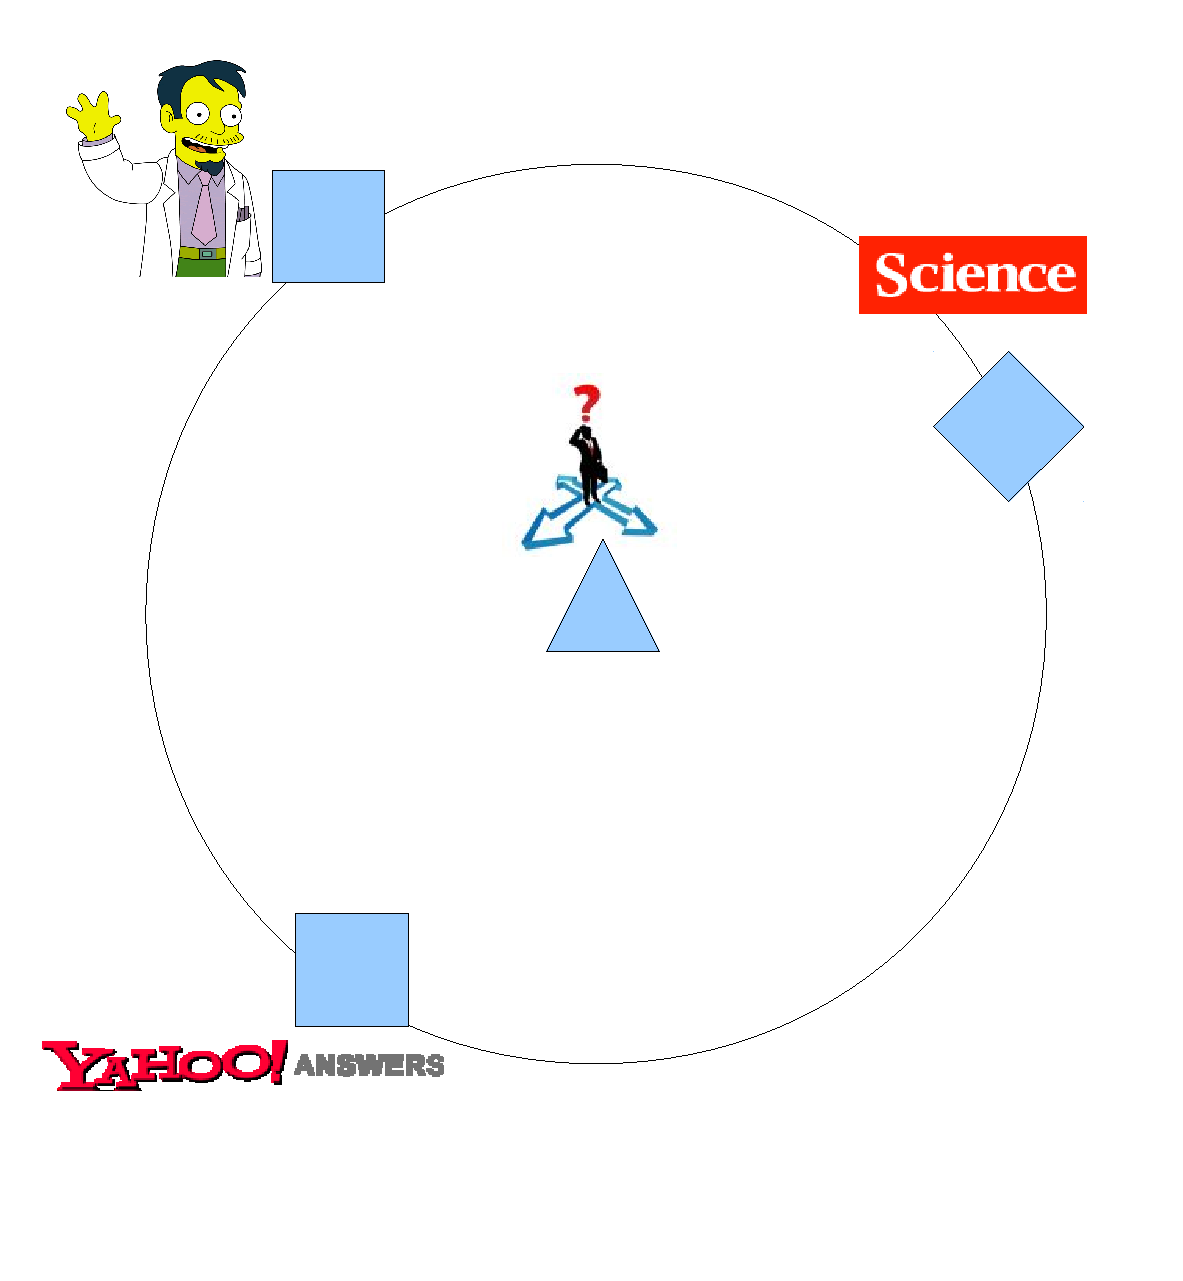
\includegraphics[width=0.7\textwidth]{Figures/medicina.eps}
\end{figure}

}


\frame{
    \frametitle{Esquema gráfico com credibilidade (baseado no \textsc{KNN})}

\begin{figure}
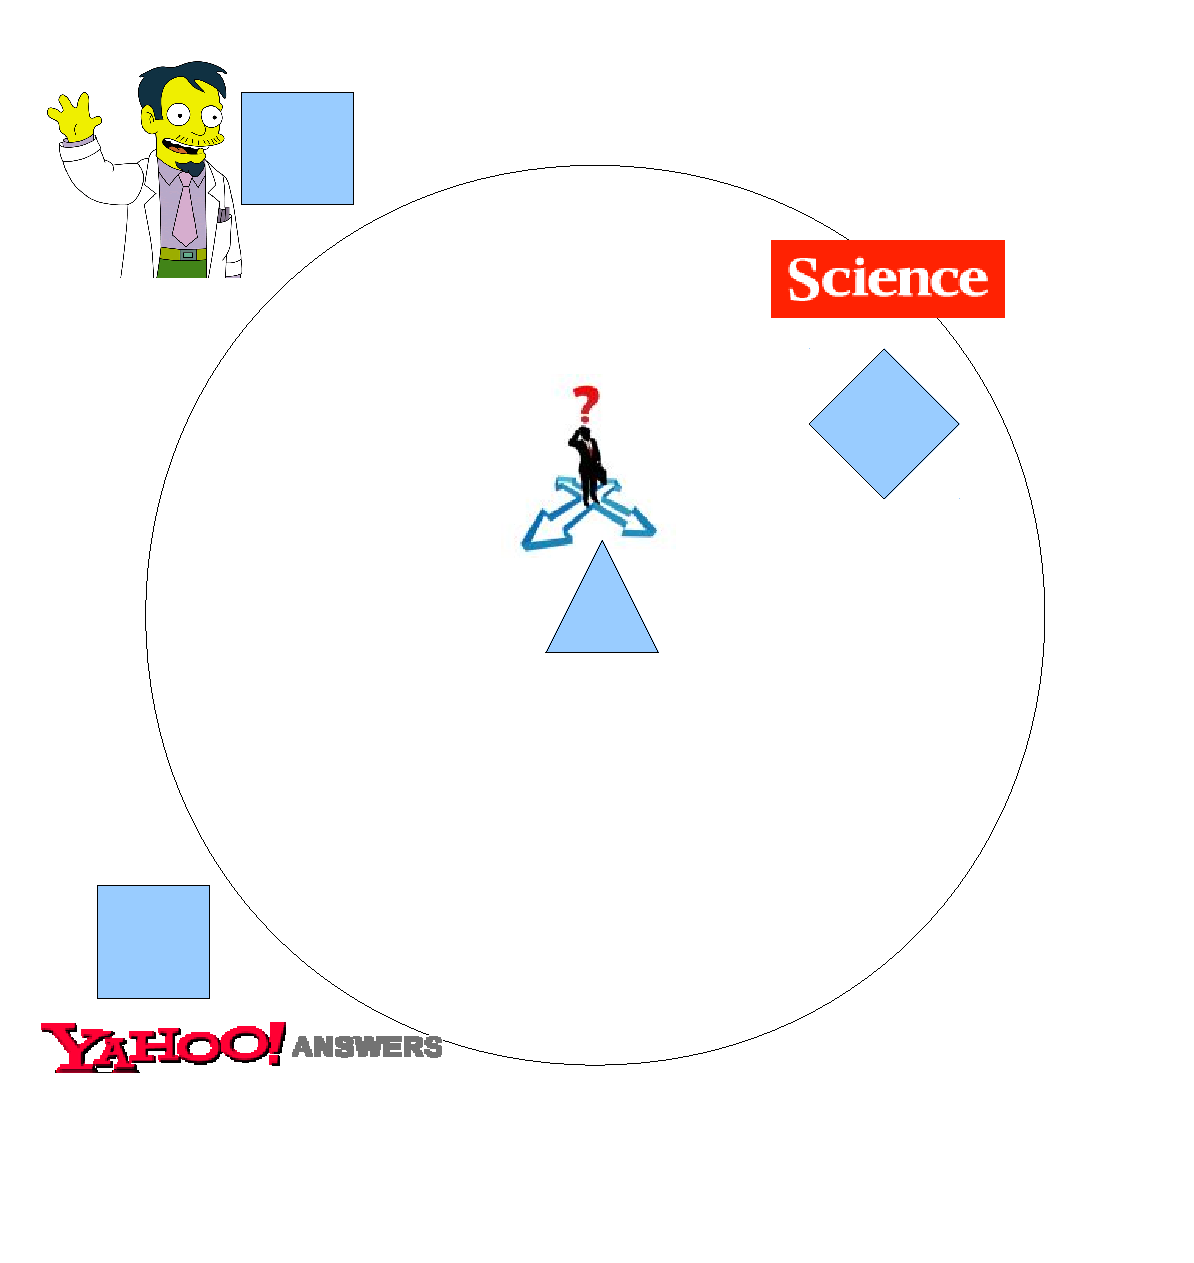
\includegraphics[width=0.7\textwidth]{Figures/medicina-cred.eps}
\end{figure}

}

\subsection{Proposta}
\frame{
    \frametitle{Proposta desse trabalho - Incorporação da Credibilidade}

\begin{figure}
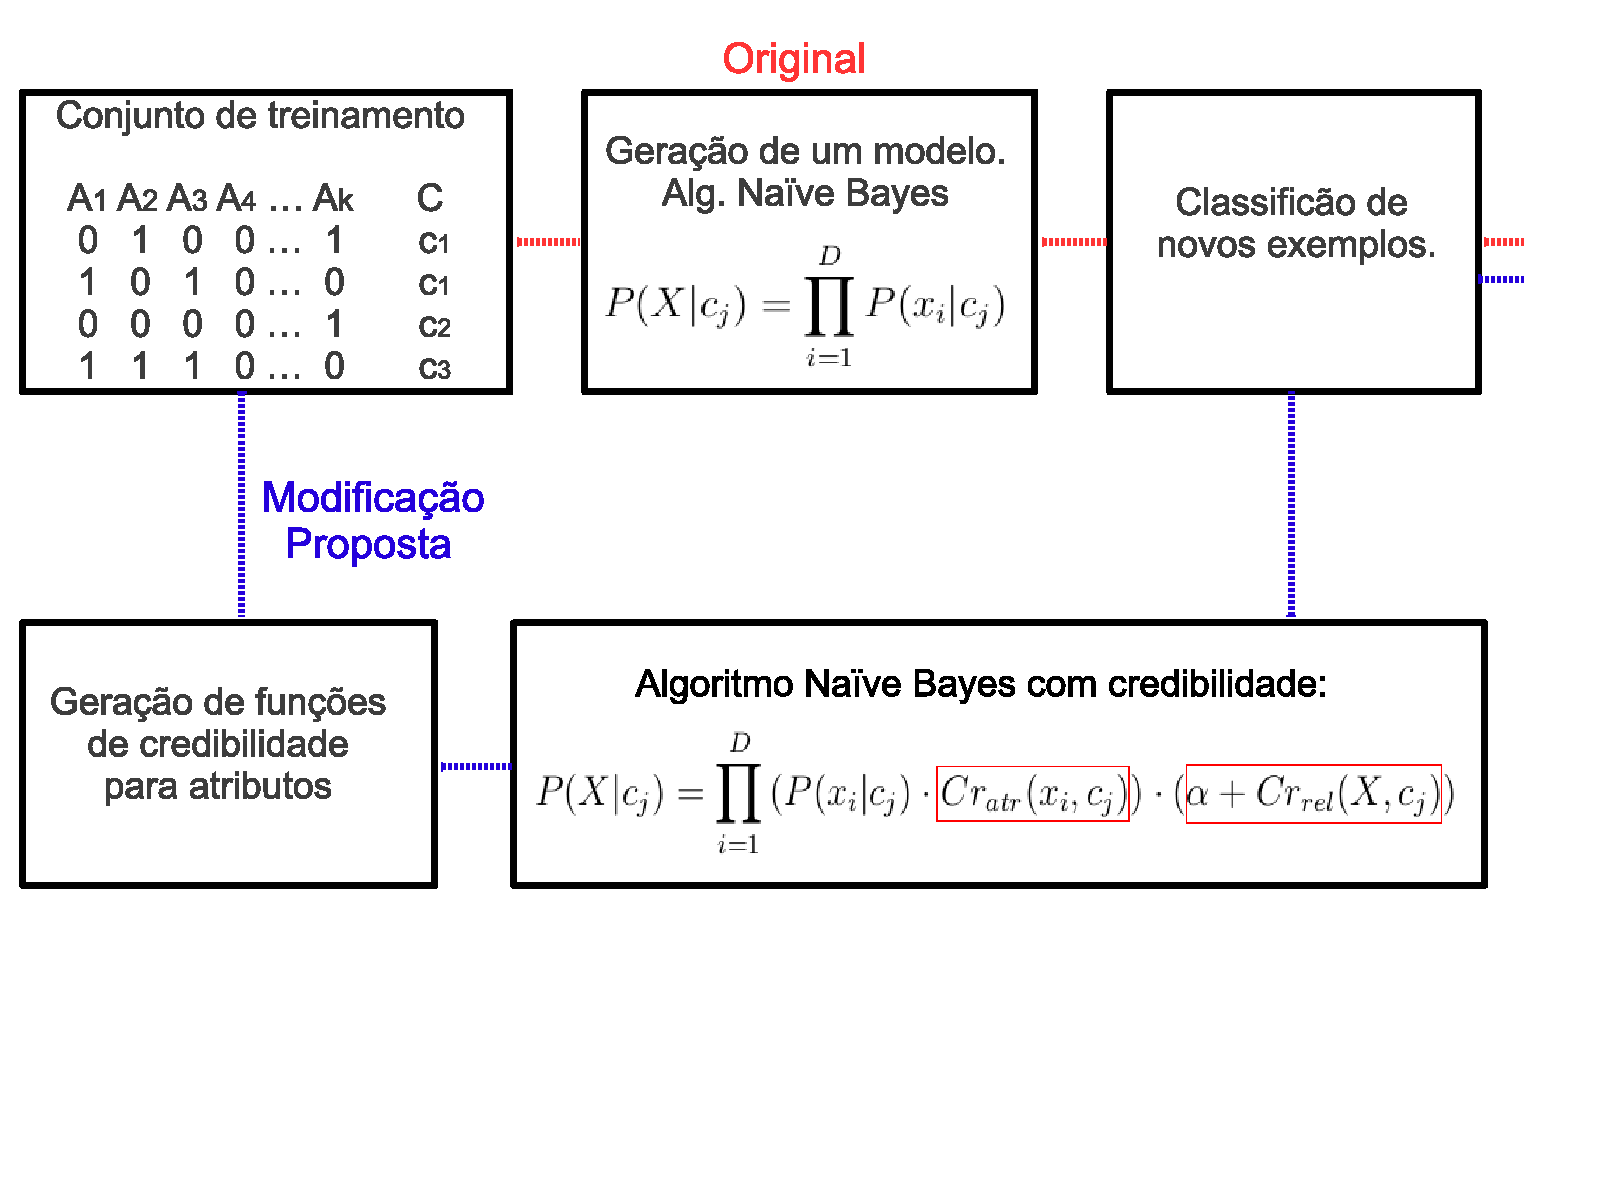
\includegraphics[width=11cm]{Figures/workflow.eps}
\caption{Classificadores que usam a credibilidade dos exemplos de treinamento.}
\end{figure}

}

\frame{
    \frametitle{Contribuições}
    \begin{center}
    \begin{itemize}

    \item Destacamos como as principais contribuições desse trabalhos:
        \vskip0.5cm

        \begin{itemize}
        \item Estudar o conceito de credibilidade, focando na tarefa de classificação.
        \vskip0.5cm

       \item Incorporar a credibilidade a classificadores, criando modelos de classificação mais robustos.
        \vskip0.5cm

       \item  Testar e analisar os impactos provenientes do uso de credibilidade.
        \vskip0.5cm

    \end{itemize}

       \item Escrevemos dois artigos para as conferências SBBD-2010 (melhor da track de Mineração) e CEC-2011.
       \item Criamos a ferramenta de visualização de Programação Genética chamada Galapagos, melhor ferramenta de visualização do GECCO-2011.
   \end{itemize}
    \end{center}

}


%%%%------------------------------------------------%%%%

\section{Classificadores e Credibilidade}
\subsection{Credibilidade}

\frame{
    \frametitle{Credibilidade - Proposta}

    \begin{itemize}

        \item A maioria dos métodos de classificação assume que todos os exemplos de treinamento devem contribuir igualmente para a criação de um modelo de classificação.
        \vskip1cm
\pause
        \item Acreditamos que a contribuição deveria variar de acordo com a confiabilidade que temos em cada um dos exemplos.
        \vskip1cm
\pause
        \item Propomos a criação de \textbf{funções de credibilidade} para medir em um valor real o quanto podemos confiar em um dado exemplo.

    \end{itemize}
}

\frame{
  \frametitle{Credibilidade}

    \begin{itemize}
        \item A credibilidade é tratada na literatura em diversos contextos diferentes.
        \vskip1cm

        \pause
        \item Definimos a credibilidade do ponto de vista de um classificador.
        \vskip1cm
        
        \pause
        \item Em geral, são estipulados fatores que influenciam na credibilidade de objeto.
        \vskip1cm
    
        \pause
        \item Definimos que fatores importantes na tarefa de classificação estão acoplados aos \textbf{atributos} e aos \textbf{relacionamentos} dos exemplos.
        \vskip1cm

    \end{itemize}
}

\frame{
    \frametitle{Credibilidade baseada nos \textbf{Atributos}}
    
    \begin{itemize}

    \item Atributos estão presentes em quase todos problemas de classificação.
    \vskip1cm

    \item Métricas de \textbf{seleção de atributos}: importantes para avaliar a contribuição de cada atributo na relação atributo-classe. 
    \vskip1cm
    
    \end{itemize}

}


\frame{

    \frametitle{Credibilidade baseada em \textbf{Atributos}}
        
        \begin{itemize}

            \item Classificação de documentos: termos \textbf{Metallica} X \textbf{Anthrax}.

\begin{figure}
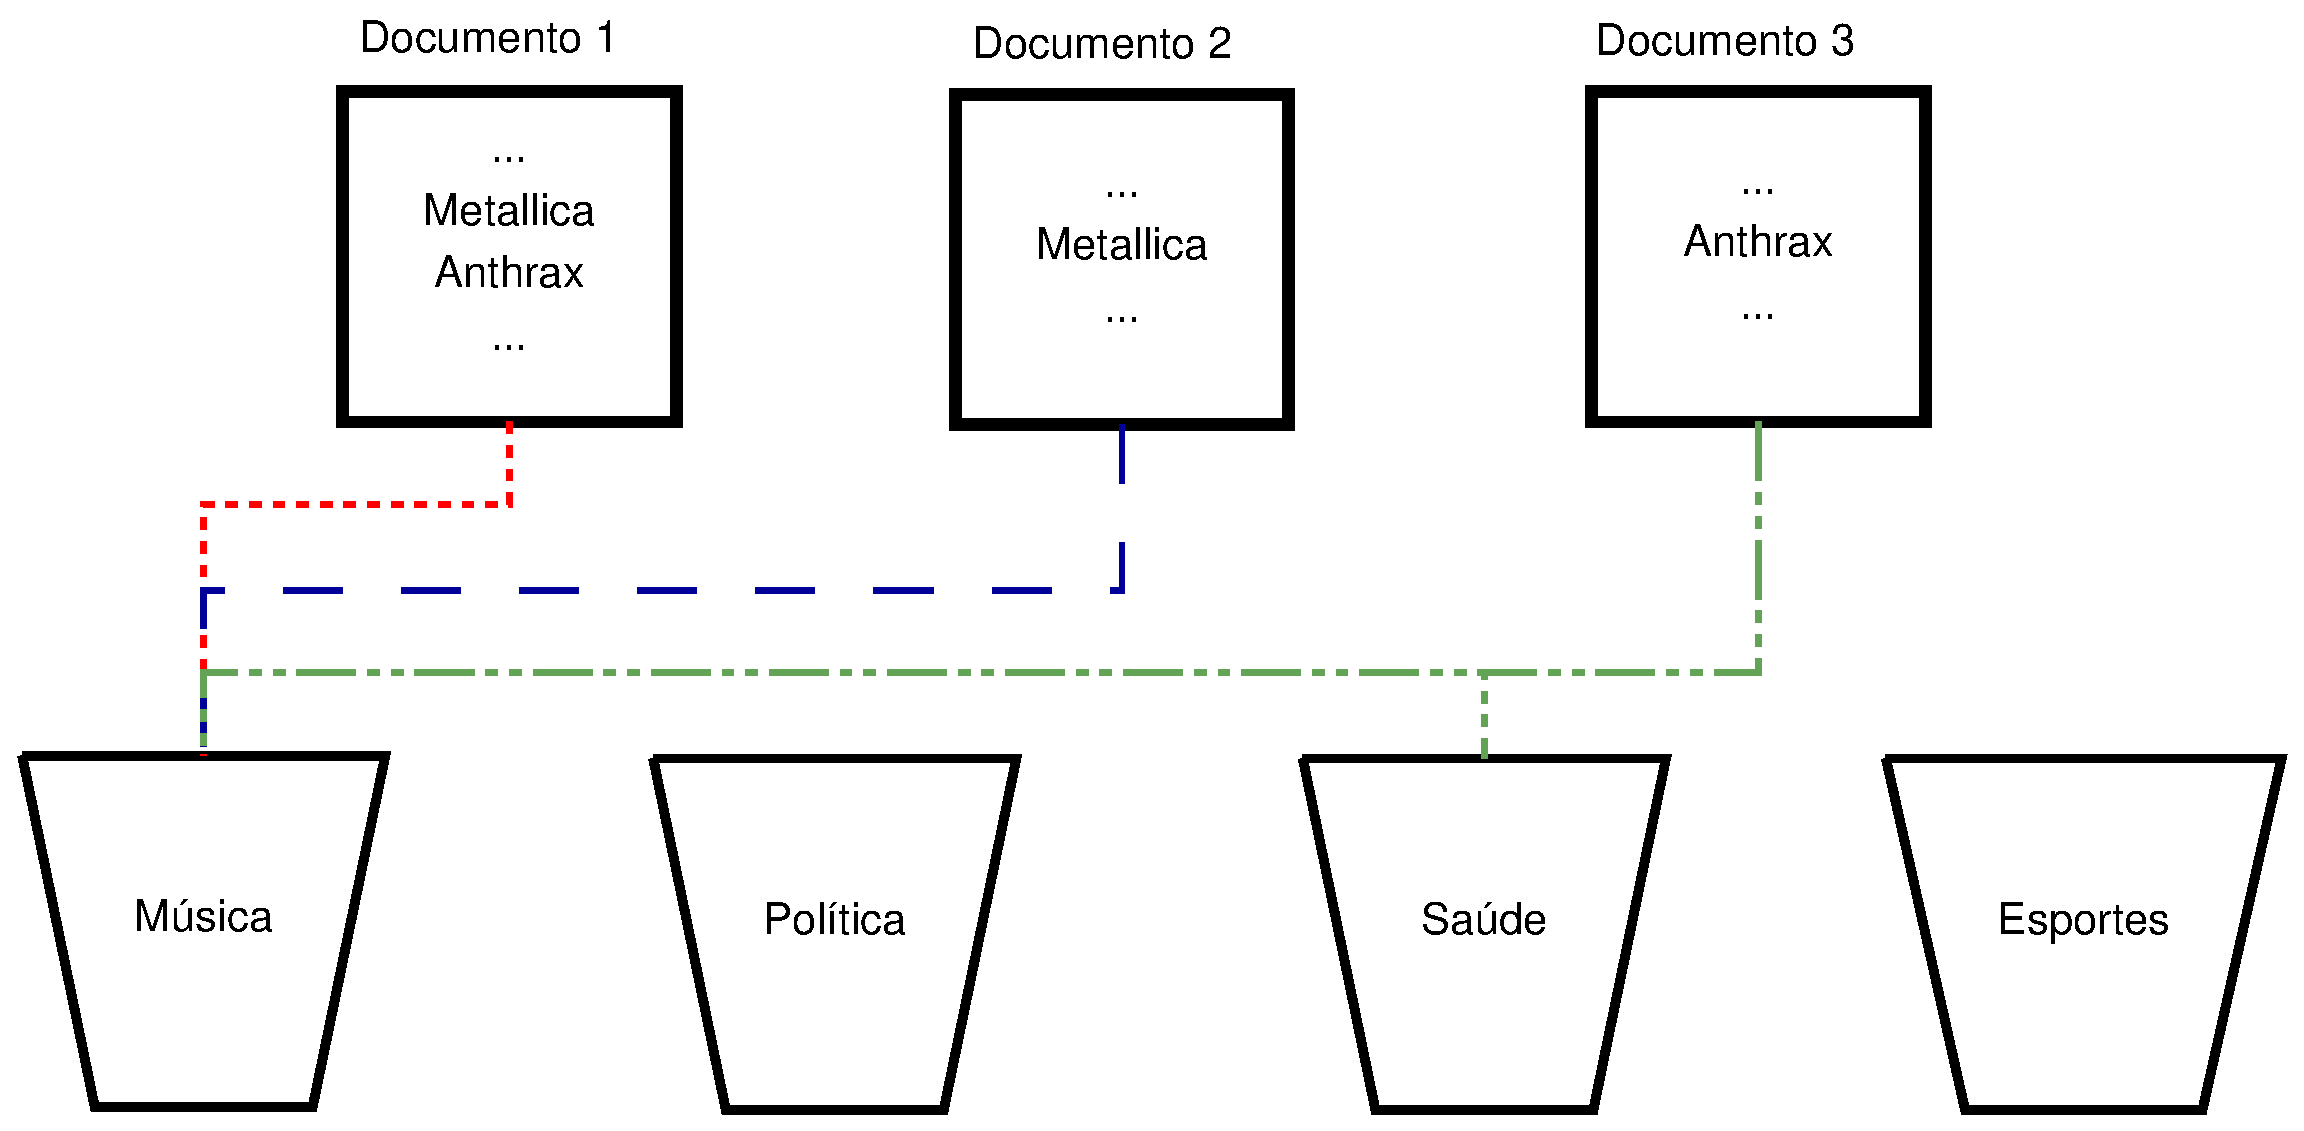
\includegraphics[width=0.8\textwidth]{Figures/termos.eps}
\end{figure}

\pause
            \item Definimos 30 métricas capazes de medir a relação atributo-classe. Exemplo:

\begin{equation*}\label{eqn::chi}
  \textsc{CHI}(x_i, c_j) = N \cdot \frac{ [ \textsc{P}(x_i|c_j) \cdot \textsc{P}(\overline{x_i}|\overline{c_j}) - \textsc{P}(x_i|\overline{c_j}) \cdot \textsc{P}(\overline{x_i}|c_j) ]^2 } {\textsc{P}(x_i) \cdot \textsc{P}(\overline{x_i}) \cdot \textsc{P}(c_j) \ \cdot \textsc{P}(\overline{c_j}) }.
\end{equation*}

\end{itemize}

}

\frame{

    \frametitle{Credibilidade baseada em \textbf{relacionamentos}}
        
        \begin{itemize}
            \item Classificação de documentos: rede de autoria.
            \item Desejamos saber a classe do documento \textit{Teste} que tem os autores \textsc{A}, \textsc{B} e \textsc{C}.

%            \item Seria mais intuitivo considerar mais importante um documento que tenha um subconjunto dos autores de \textit{Teste}?
%            \item Seria que um documento com todos os mesmos autores deveria ser mais importante que um que não contém nenhum autor em comum?

\begin{figure}
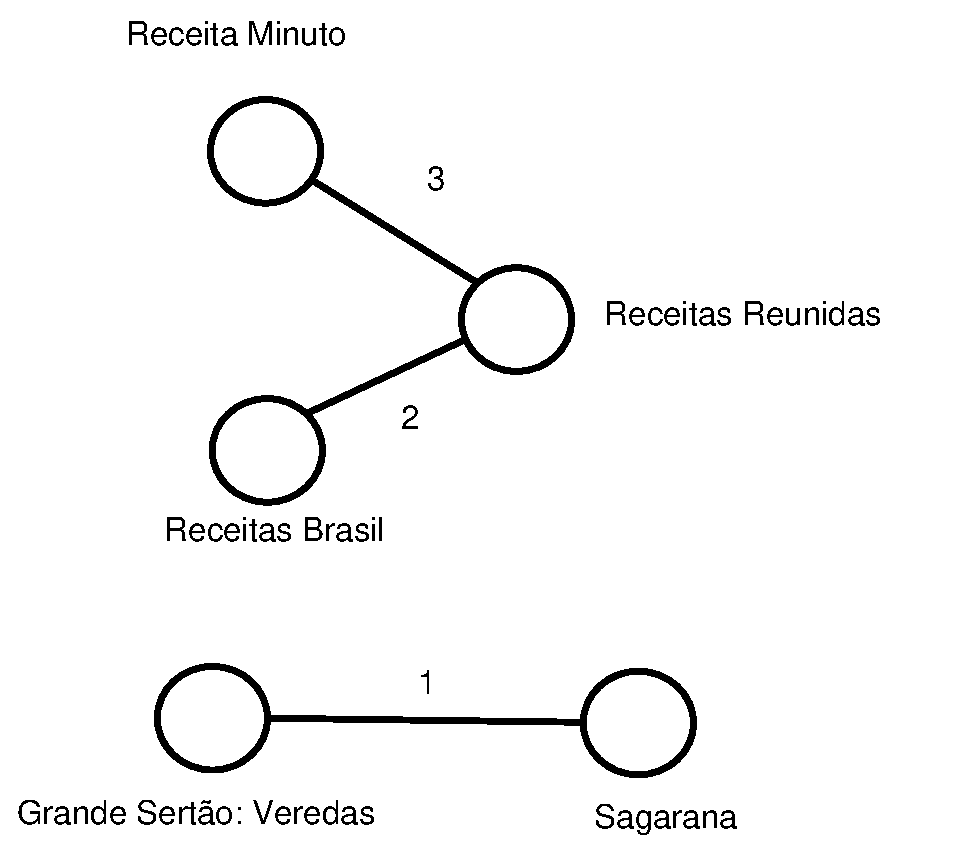
\includegraphics[width=0.4\textwidth]{Figures/grafo-livros.eps}
\end{figure}

\pause
            \item Utilizamos 16 métricas da área de Redes Complexas que mensuram características estruturais de grafos que podemos formar a partir desses relacionamentos. Exemplo: Número de vizinhos.
        \end{itemize}
}

%%%%----------------------------------------------%%%%
%%%%----------------------------------------------%%%%

\frame{
    \frametitle{Classificadores}

    \begin{itemize}

        \item Podemos incorporar a credibilidade em qualquer algoritmo de classificação.
        \vskip1cm

        \pause
        \item Nesse trabalho focamos em dois:
            \vskip0.5cm
            \begin{itemize}
                \item \textit{Naïve Bayes}: Bom compromisso entre tempo de execução e desempenho. Boas linhas de base para classificação de documentos.
                \vskip0.5cm

                \item \textsc{KNN}: Já apresenta um modelo simplificado de credibilidade. Boas linhas de base para atributos categóricos e bioinformática.
                \vskip0.5cm

            \end{itemize}

    \end{itemize}

}

\subsection{Naïve Bayes}
\frame{
    \frametitle{\textit{Naïve Bayes} - Incorporando Credibilidade nos classificadores}

\begin{itemize}

    \item <1-> \textit{Naïve Bayes} consiste em:

\begin{equation*}\label{eqn::max_pcgivenx}
   P(c_{j}|X) > P(c_{k}|X) \;\;\;\;\;\forall k,\; 1 \le k \le M, \; k \not= j,
\end{equation*}

\item <2-> Para cada classe calculamos:

\begin{equation*}\label{eqn::classindependence}
   P(X|c_{j}) = \prod^{D}_{i=1}{P(x_i|c_j) }
\end{equation*}

\item <3-> Credibilidade:

\begin{equation*}\label{eqn::nbcredcompleta}
P(X|c_{j}) = \prod^{D}_{i=1}{(P(x_i|c_j) \cdot Cr_{atr}(x_i,c_j)) \cdot (\alpha + Cr_{rel}(X,c_j)) } 
\end{equation*}

\end{itemize}

}

\subsection{KNN}
\frame{
    \frametitle{\textsc{KNN} - Incorporando Credibilidade nos classificadores}

    \begin{figure}[ht]
        \centering
        \subfigure[a][\textsc{KNN} original]{
            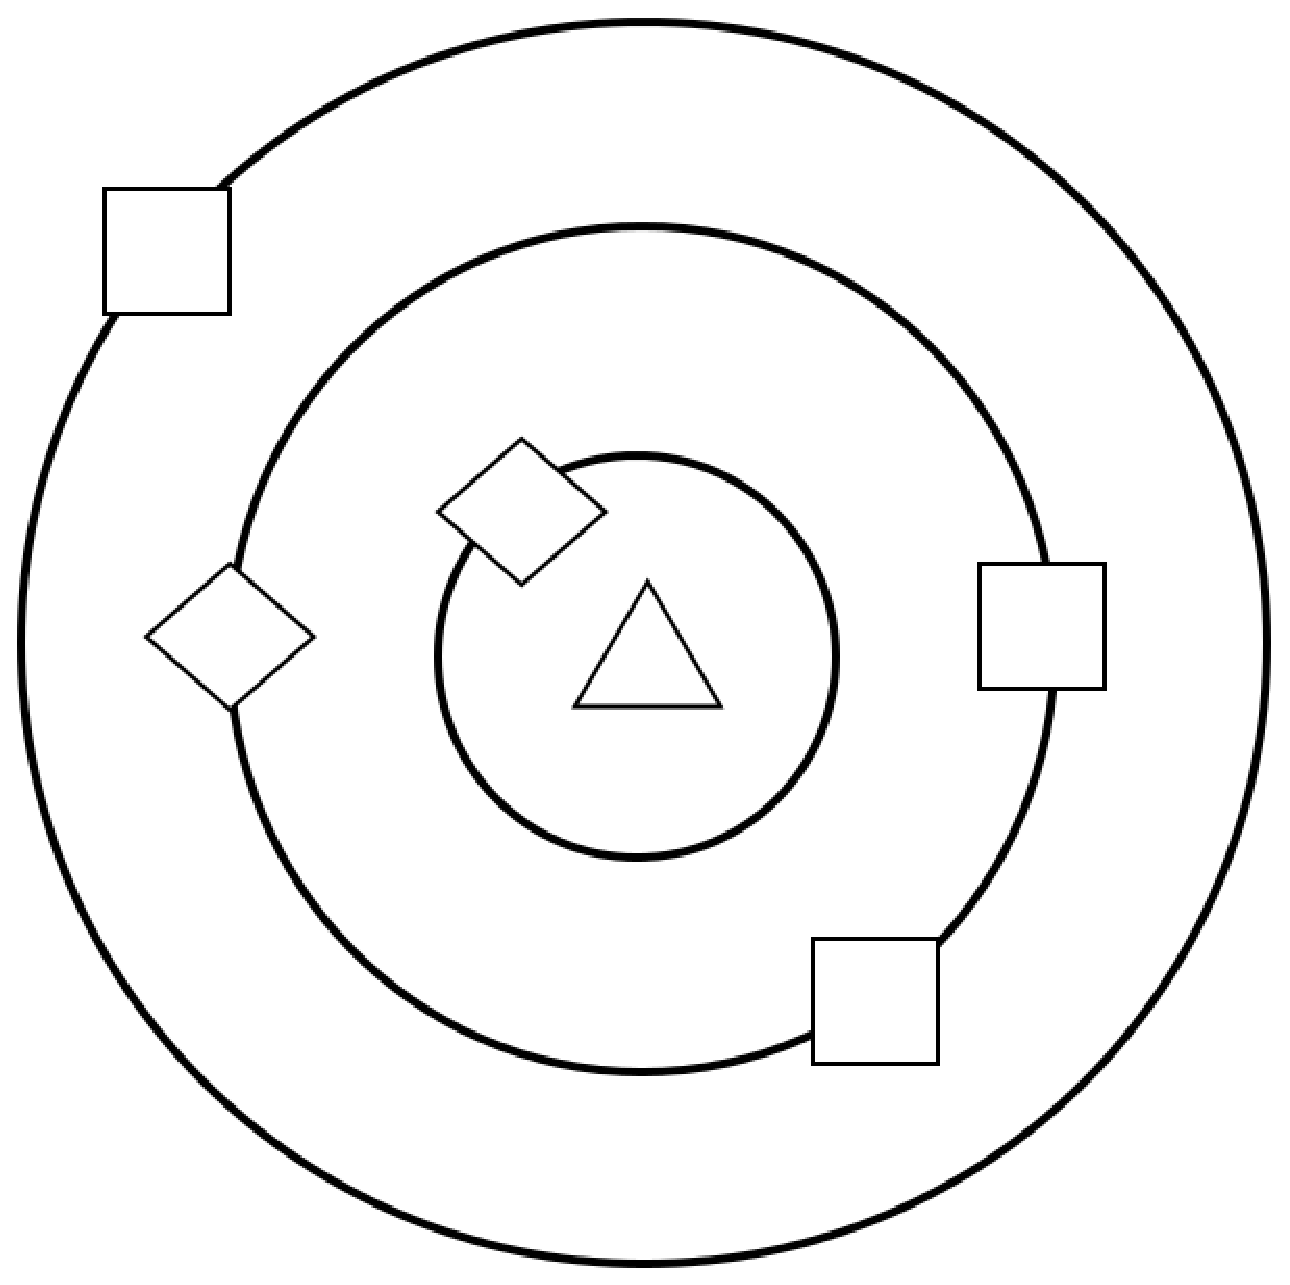
\includegraphics[width=0.35\textwidth]{Figures/knn.eps}
        }
        \pause
        \subfigure[b][\textsc{KNN} com credibilidade]{
            %    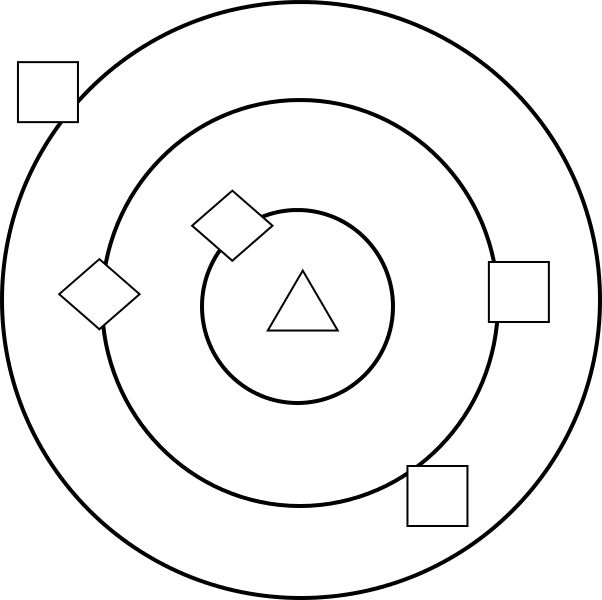
\includegraphics[width=0.5\textwidth]{figures/knncred.png}
             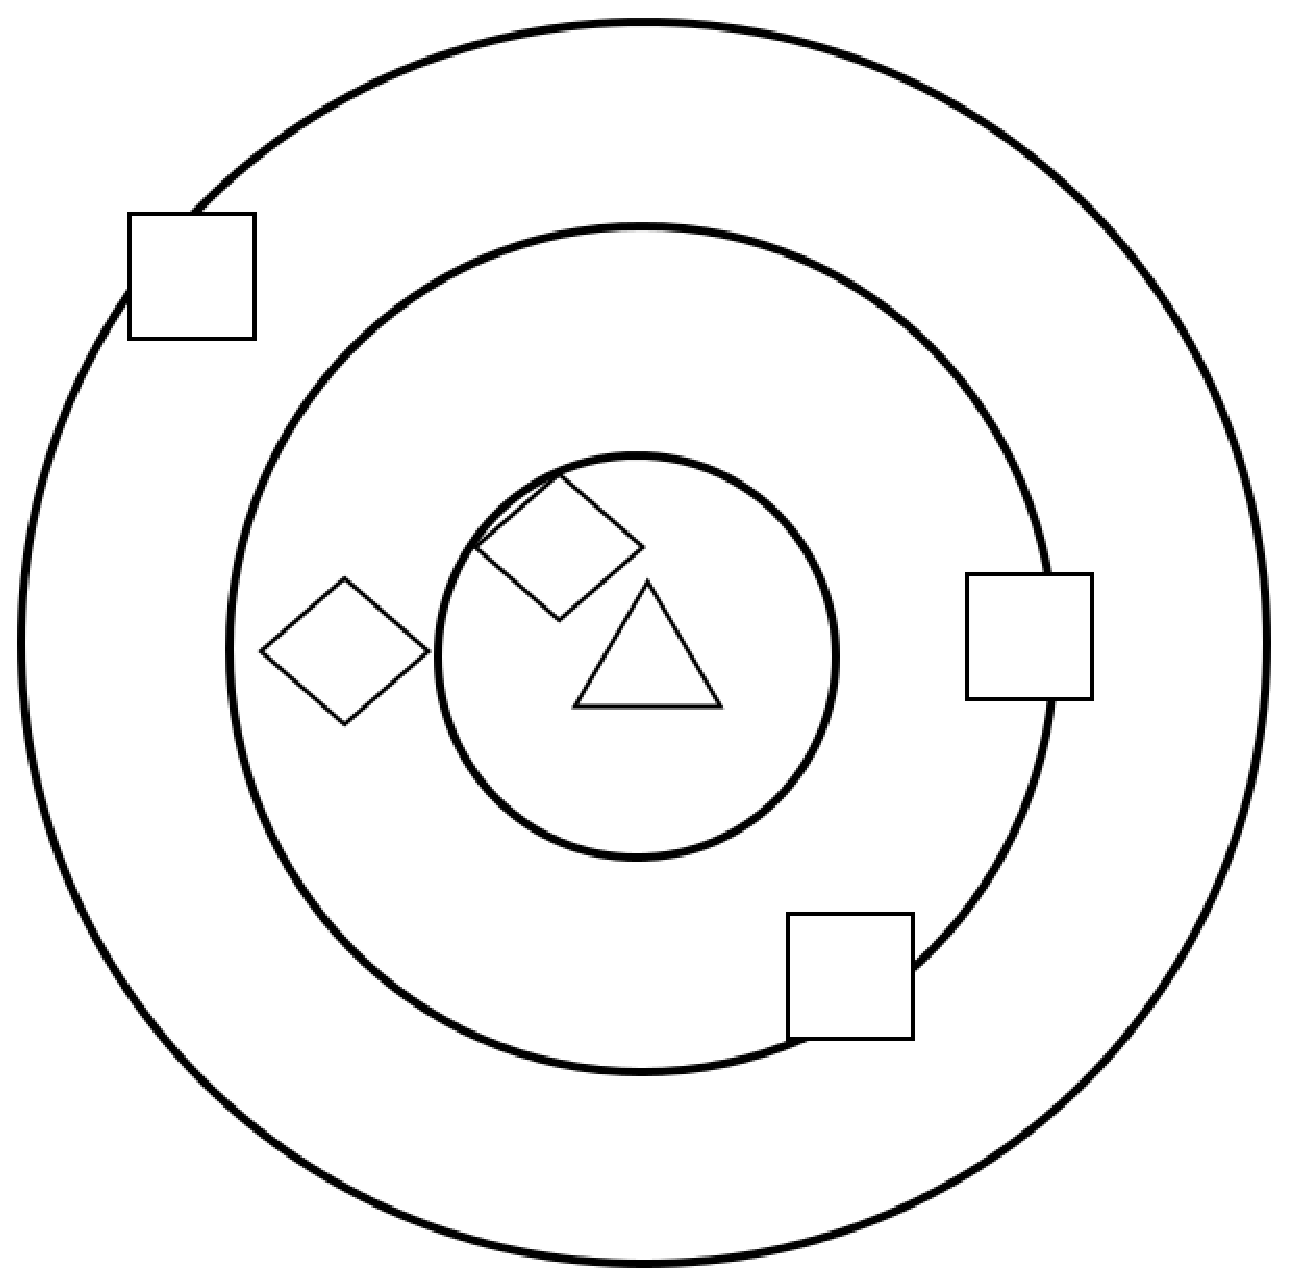
\includegraphics[width=0.35\textwidth]{Figures/knn_aproxima.eps}
        }
%        \caption{Em (a) temos o algoritmo original dos $K$ vizinhos mais próximos e em (b) temos um possível resultado da utilização da credibilidade conjuntamente ao \textsc{KNN}.  
%        \label{fig::KNNantesedepois}}
    \end{figure}

    \pause
    \begin{equation}\label{eqn::distancia_texto}
        dist(X_1, X_2) = (-1) \times \sum\limits_{1 < i < D} \frac{ x_{i1} \cdot w_{i1} \cdot x_{i2} \cdot w_{i2} }{ ||X_1|| \cdot ||X_2|| }
    \end{equation}

    \pause
    \begin{equation*}\label{eqn::distancia_texto_cat}
    \hspace{-1cm}
        dist(X_1, X_2) = (-1) \times \sum\limits_{1 < i < D}\frac{  Cr_{atr}(t_{i1}, c_{X_2}) \cdot x_{i1} \cdot w_{i1} \cdot x_{i2} \cdot w_{i2} }{ ||X'_1|| \cdot ||X_2|| } \times  \frac{1}{(\alpha + Cr_{rel}(X_1, class_{X_2}) )}
    \end{equation*}
}

\frame{

    \frametitle{Como escolher uma função de credibilidade para cada fator?}
        
        \begin{itemize}
            \item Vimos que modelamos 30 métricas para os atributos e 16 para os relacionamentos.
            \vskip1cm
            \pause
            \item Qual a melhor forma de relacionar as métricas de atributos? E as de relacionamento?
            \vskip1cm
            \pause
            \item Utilizamos \textbf{Programação Genética} para evoluir nossas funções de credibilidade.
            \vskip1cm
            \pause
            \item Justificativas: robustez, praticidade, método de otimização.
        \end{itemize}
}

%%%%------------------------------------------------%%%%
%%%%------------------------------------------------%%%%


\section{PG para Estimar Credibilidade}
\subsection{Geral}

\frame{
    \frametitle{Programação Genética (\textbf{PG})}

    \begin{itemize}
    
        \item \textsc{PG} é um algoritmo inspirado na teoria da evolução de Darwin.
        \vskip1cm

        \item Indivíduos são inicialmente criados e evoluídos ao passar das gerações.
        \vskip1cm

        \pause
        \item A população de indivíduos de uma geração nova tende a ser melhor (mais bem preparada) para que geração anterior.
        \vskip1cm

        \item Métodos de otimização que lida bem com ruídos.
        \vskip1cm
    \end{itemize}

}

\frame{
    \frametitle{Exemplos de indivíduos}

   \begin{figure}[!ht]
        \centering
            \subfigure[][Função 1:\newline $\textsc{GINI}(x)^{\textsc{CC}(x,c)}$]{
                \includegraphics[width=0.20\textwidth]{Figures/gp1c2.eps}
            }
            \hskip1cm
            \subfigure[][Função 2: \scriptsize \newline \hspace*{-7mm}$(\textsc{AM}(x,c) + \textsc{P}(x|c)) \% (\textsc{IG}(x,c))$]{
                \includegraphics[width=0.25\textwidth]{Figures/gp2c2.eps}
            }
            \hskip1cm
            \subfigure[][Função 3:\newline \hspace*{4mm} $\textsc{GINI}(x)^{(\textsc{AM}(x,c)\ + \ \textsc{P}(x|c))}$]{
                \includegraphics[width=0.25\textwidth]{Figures/gp3c2.eps}
            }
            \\         
            \subfigure[][Função 4:\newline \hspace*{-3.5mm}$\textsc{Bib}(X,c) - {\textsc{Hub}(x,c)}$]{
                \includegraphics[width=0.20\textwidth]{Figures/gp1c_grafos2.eps}
            }
            \hskip2cm
            \subfigure[][Função 5:\newline \hspace*{-4mm} $\textsc{Bib}(X,c) - \textsc{PR}(X,c) $]{
                \includegraphics[width=0.20\textwidth]{Figures/gp2c_grafos2.eps}
            }
%    \caption{Três possíveis funções de credibilidade de atributos.}
    \label{fig::gps1}
    \end{figure}
}

 \frame{

    \frametitle{Programação Genética (\textbf{PG})}

    \begin{figure}
    \centerline{\includegraphics[width=1.15\textwidth]{Figures/gpwf_new2.eps}}
    \caption{Fluxograma de um algoritmo de Programação Genética}
    \end{figure}
}

\subsection{Representação}

\frame{
    \frametitle{Exemplos de indivíduos e operações}

   \begin{figure}[!ht]
        \centering
            \subfigure[][Função 1:\newline \hspace*{6mm}$\textsc{GINI}(x)^{\textsc{CC}(x,c)}$]{
                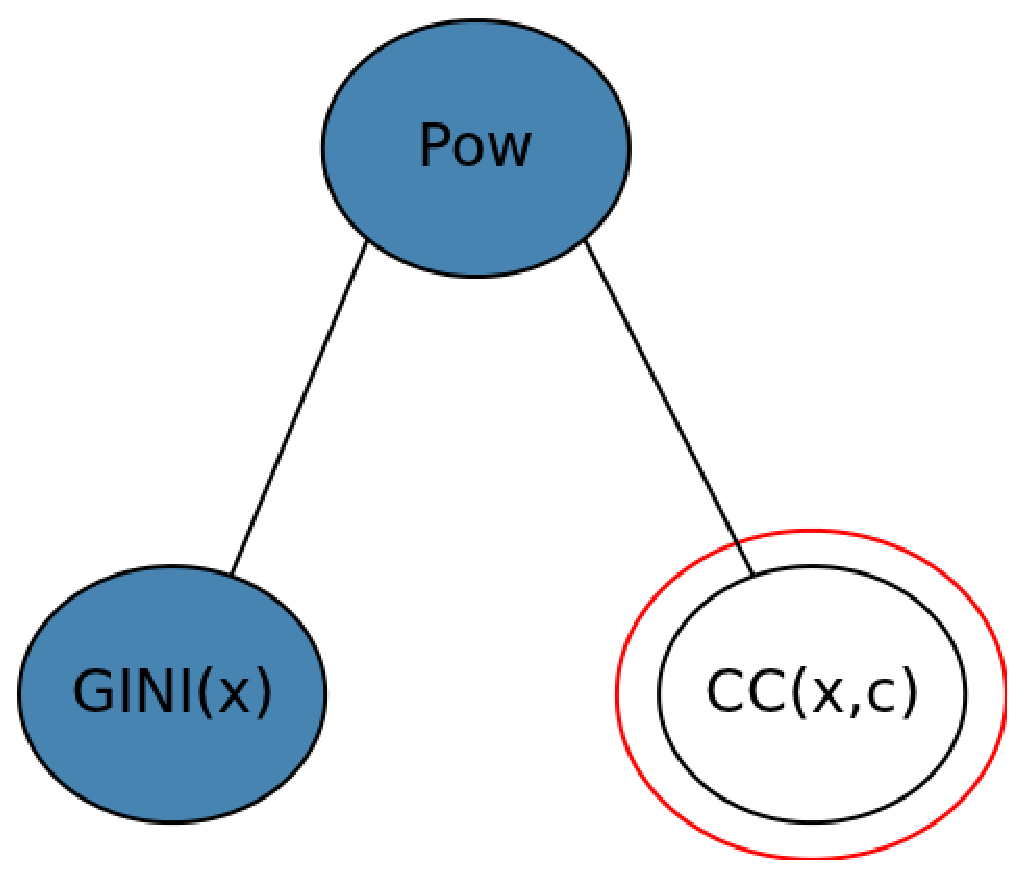
\includegraphics[width=0.25\textwidth]{Figures/gp1c.eps}
            }
            \hskip0.1cm
            \subfigure[][Função 2: \scriptsize \newline \hspace*{-5mm}$(\textsc{AM}(x,c) + \textsc{P}(x|c)) \% (\textsc{IG}(x,c))$]{
                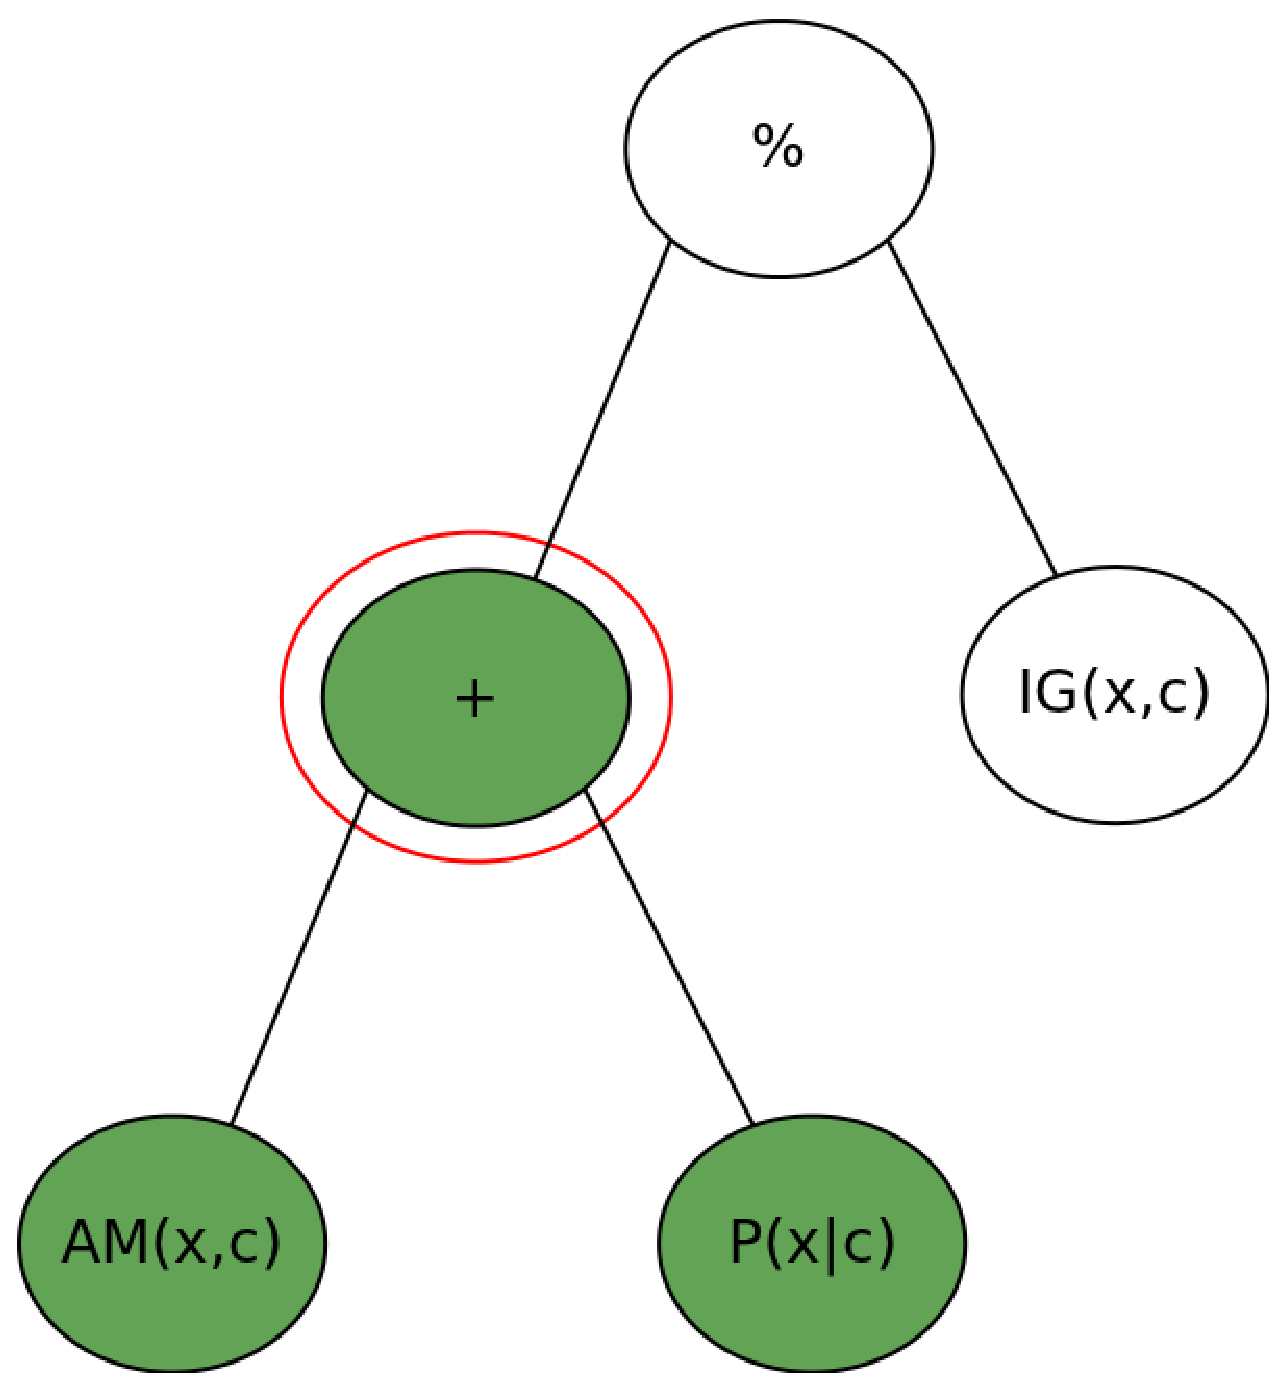
\includegraphics[width=0.33\textwidth]{Figures/gp2c.eps}
            }
            \hskip0.1cm
            \subfigure[][Função 3:\newline \hspace*{4mm} $\textsc{GINI}(x)^{(\textsc{AM}(x,c)\ + \ \textsc{P}(x|c))}$]{
                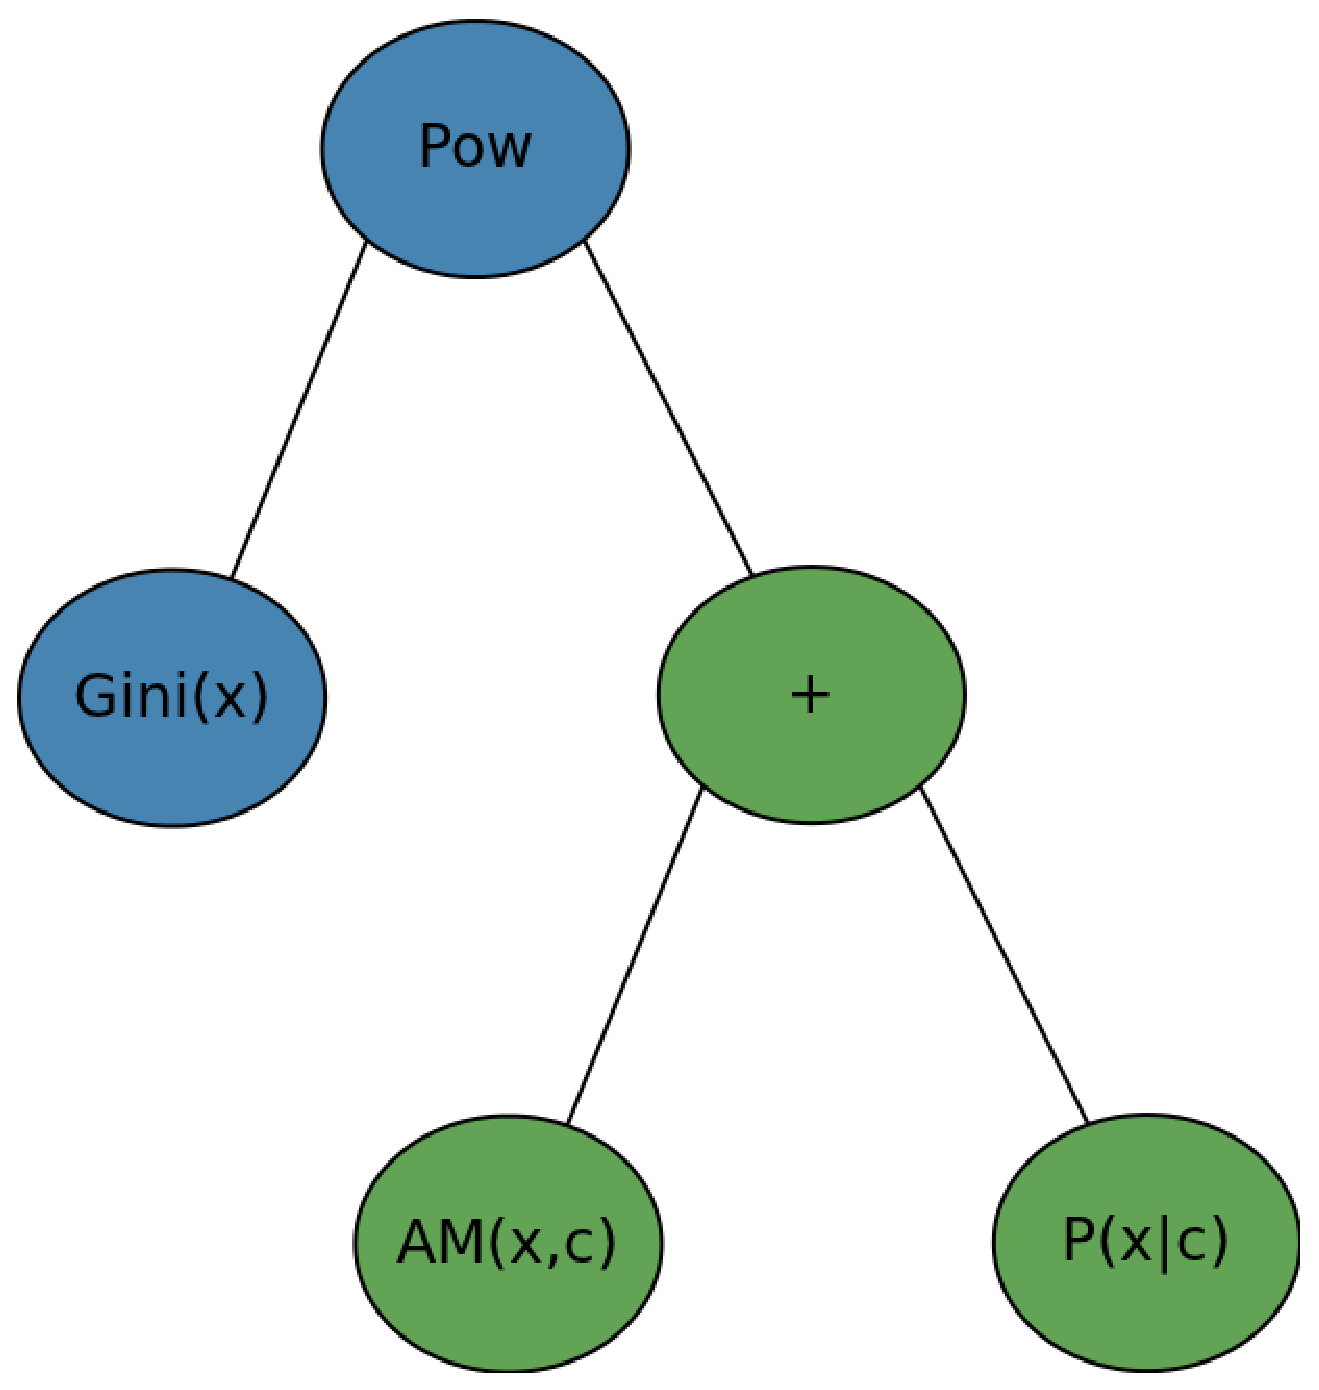
\includegraphics[width=0.33\textwidth]{Figures/gp3c.eps}
            }
    \caption{Três possíveis funções de credibilidade de atributos.}
    \label{fig::gps1}
    \end{figure}

}


 \frame{

    \frametitle{Programação Genética (\textbf{PG})}

    \begin{figure}
    \centerline{\includegraphics[width=1.15\textwidth]{Figures/gpwf_new2.eps}}
    \caption{Fluxograma de um algoritmo de Programação Genética}
    \end{figure}
}


\frame{
    \frametitle{Exemplos de indivíduos e operações}

   \begin{figure}[!ht]
        \centering
            
    \subfigure[][Função 1:\newline \hspace*{6mm}$\textsc{Bib}(X,c) - {\textsc{Hub}(x,c)}$]{
        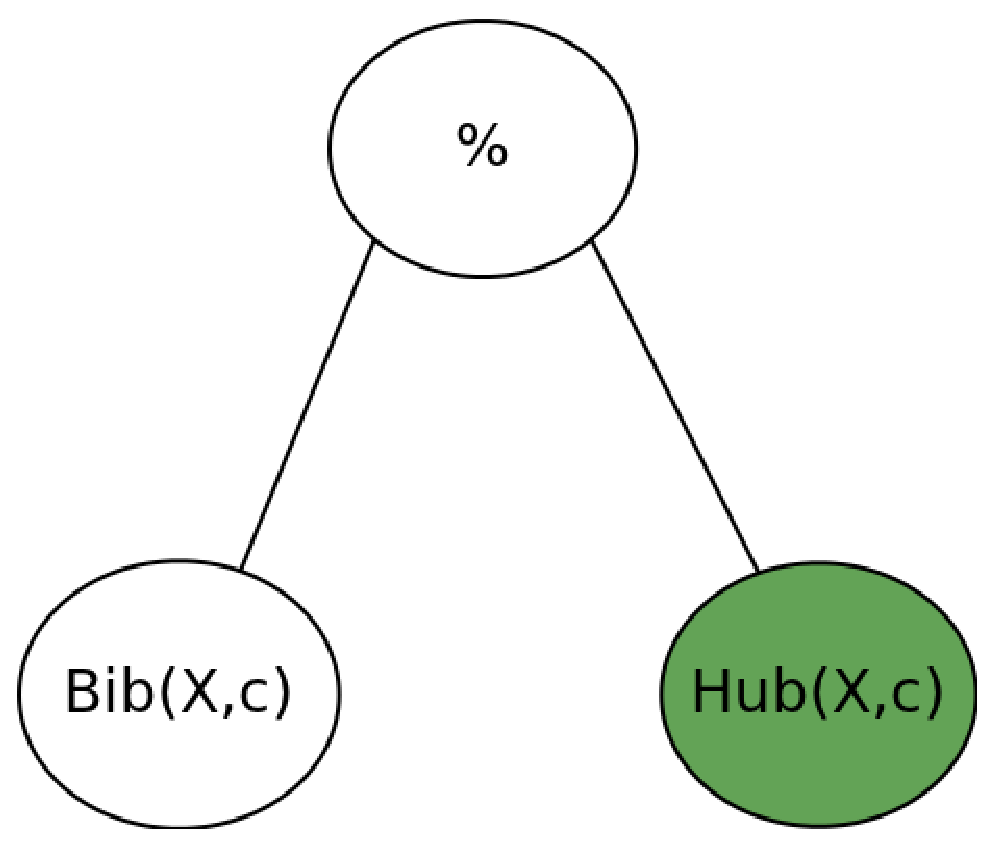
\includegraphics[width=0.30\textwidth]{Figures/gp1c_grafos.eps}
    }
    \hskip1cm
    \subfigure[][Função 2:\newline \hspace*{5mm} $\textsc{Bib}(X,c) - \textsc{PR}(X,c) $]{
        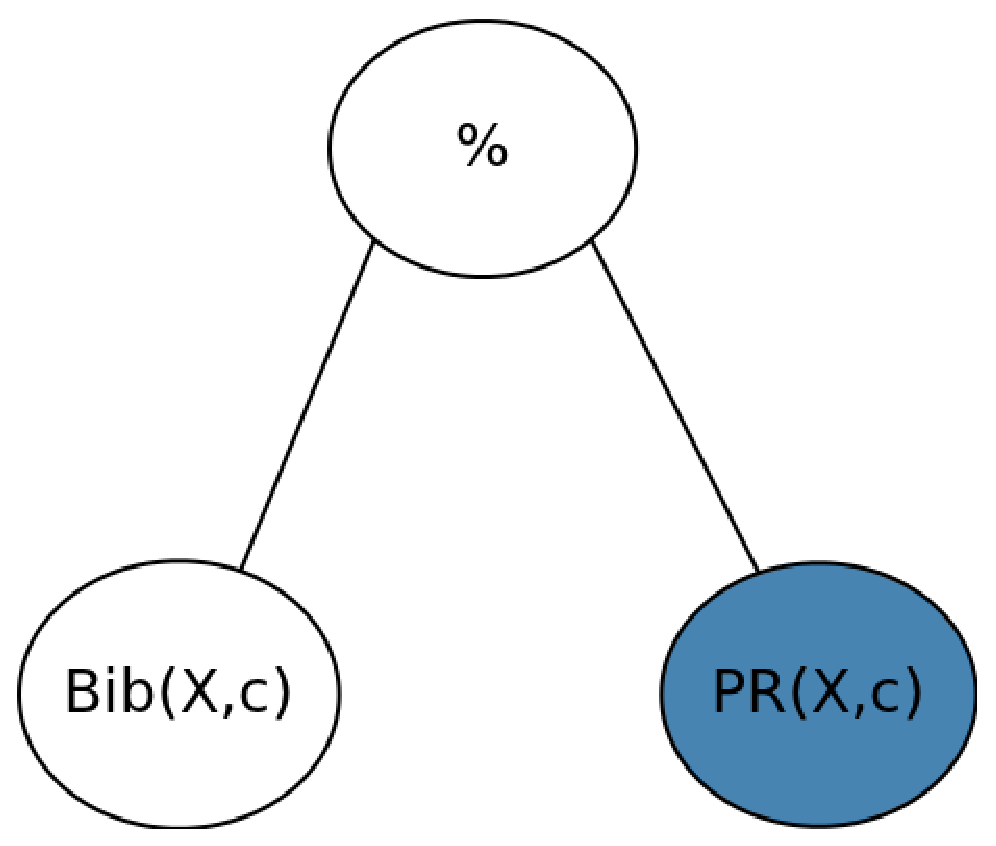
\includegraphics[width=0.30\textwidth]{Figures/gp2c_grafos.eps}
    }
    \caption{Duas possíveis funções de credibilidade de relacionamentos.}
    \label{fig::gps1}
    \end{figure}
}

 \frame{

    \frametitle{Programação Genética (\textbf{PG})}

    \begin{figure}
    \centerline{\includegraphics[width=1.15\textwidth]{Figures/gpwf_new2.eps}}
    \caption{Fluxograma de um algoritmo de Programação Genética}
    \end{figure}
}

\subsection{Fitness}

\frame{
  \frametitle{\textit{Fitness}}

  \begin{itemize}

  \item <1-> Precisão = $\textsc{P} =  \frac{\# \text{de exemplos da classe c corretamente classificados como classe c}} {\# \: \text{ total de exemplos classificados como classe c}}$
  \item <1-> Revocação = $\textsc{R} = \frac{\# \: \text{de exemplos da classes c corretamente classificados como classe c}}{\# \: \text{de exemplos existentes na classe c}}$
  
  \item <1-> \textit{Fitness}: $\text{F}_1 = \frac{2 \times P \times R}{(P + R)}$
  
  \vskip-1cm
  \item <2-> Micro-$F_1$: Considera todas as classes de apenas uma vez.

  \item <2-> Macro-$F_1$: Considera a $F_1$ de cada classe e realiza uma média ao final.

    \begin{itemize}
        \item Sujeito a valores ruins, se uma das classes for muito difícil.
    \end{itemize}

 \end{itemize}
}


 \frame{

    \frametitle{Programação Genética (\textbf{PG})}

    \begin{figure}
    \centerline{\includegraphics[width=1.15\textwidth]{Figures/gpwf_new2.eps}}
    \caption{Fluxograma de um algoritmo de Programação Genética}
    \end{figure}
}

%\frame{
%  \frametitle{\textit{Fitness} - Algoritmo}
%
%\algrenewcommand\algorithmicforall{\textbf{Para Cada}}
%\algrenewcommand\algorithmicdo{\textbf{Faça}}
%\algrenewcommand\algorithmicfunction{\textbf{Função}}
%\algrenewcommand\algorithmicif{\textbf{Se}}
%\algrenewcommand{\algorithmicreturn}{\textbf{retorna}} %% nao sei pq nao funciona, pesquisar depois
%
%\begin{algorithm}[H]
%\centering
%\caption{Calula Fitness.}
%\label{alg::fitness}
%\begin{algorithmic}[!h]
%{
%\scriptsize
%\Function{CalculaFitness}{$individuo$}
%  \State  
%  \State \textit{Credibilidade dos atributos:}
%  \If{Utilizando Credibilidade Baseada em Atributos}
%  \ForAll{$x \in \mathbb{A}$}
%    \ForAll{$c \in \mathbb{C}$}
%      \State $f_a(x,c) \gets eval(individuo_{attrs}, x, c)$
%    \EndFor
%  \EndFor
%  \EndIf
%  \State
%  
%  \State \textit{Credibilidade dos relacionamentos:}
%  \If{Utilizando Credibilidade Baseada em Relacionamentos}
%  \ForAll{$r \in \mathbb{R}$}
%    \ForAll{$e \in \mathbb{E}$}
%        \ForAll{$c \in \mathbb{C}$}
%            \State $f_r(r,e,c) \gets eval(r,individuo_{rel}, e, c)$
%        \EndFor
%    \EndFor
%  \EndFor
%  \EndIf
%  \State
%  \State \textit{Avaliação da Fitness:}
%  \State fitness $\gets$ \textsc{F$_1$}(\textsc{Classifier}$(\mathbb{T}, \mathbb{E}, \mathbb{C}, f_a, f_r)$)
%  \State \textbf{return} fitness
%\EndFunction
%}
%\end{algorithmic}
%\end{algorithm}
%
%}

\section{Experimentos}
\subsection{Configurações}

\frame{
    \frametitle{Descrição Geral dos Experimentos}

    \begin{itemize}

        
        \item Realizamos experimentos em 3 conjuntos de bases de dados: documentos, atributos categóricos, bioinformática.
        \vskip1cm
        
        \pause
        \item Em todos utilizamos validação cruzada e \textit{teste-t} de significância estatística.
        \vskip1cm

        \pause
        \item Em todos utilizamos a mesma configuração de parâmetros para o algoritmo de Programação Genética.
        \vskip1cm
    \end{itemize}


}

\frame{
  \frametitle{Experimentos - Metodologia}

\begin{itemize}
\item Todos os experimentos realizados com validação cruzada.

\begin{figure}[h!]
  \centering
  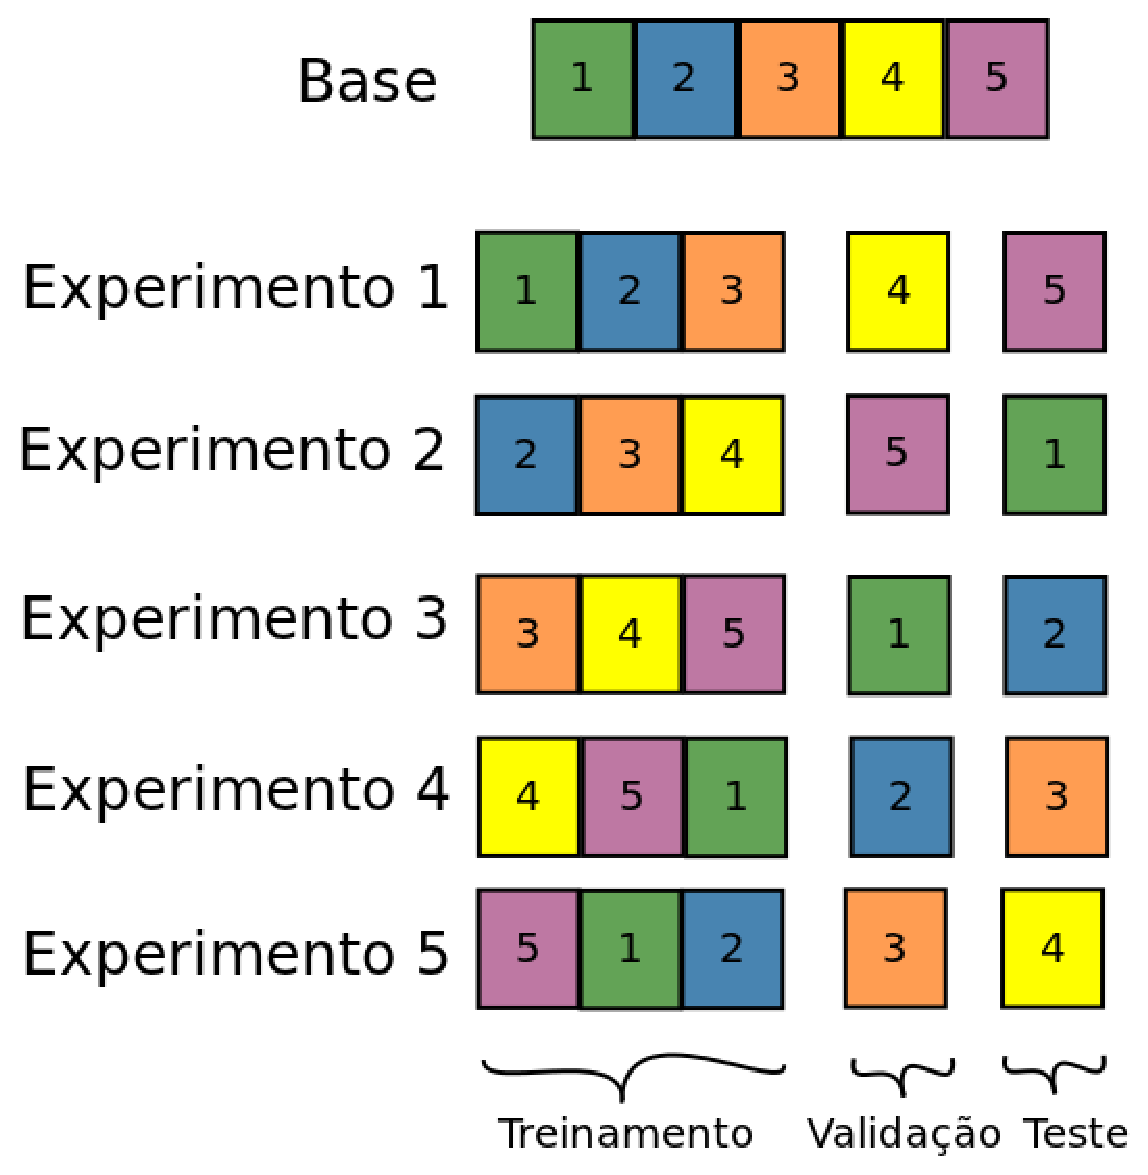
\includegraphics[width=0.40\textwidth]{Figures/cv.eps}
 \caption{Modelo de Validação Cruzada com 5 partições.}
\label{fig::cv}
\end{figure}

\item Resultados exibidos com teste $t$ e 99\% de confiança.
\end{itemize}

}

\frame{
    \frametitle{Experimentos - Parâmetros}

    \begin{itemize}
        \item Os parâmetros usados foram:


    \begin{table}[b]
        \centering
        \caption{Principais parâmetros utilizados no \textsc{PG}.}
    \label{tab::parametros}
    \begin{tabular}{lc}
    \toprule 
        \textbf{Parâmetro} & \textbf{Valor}\tabularnewline
        \midrule
        \hline
        Tamanho da População & 100\tabularnewline
        \hline 
        Número de Gerações & 100\tabularnewline
        \hline 
        Tipo de Seleção & Torneio\tabularnewline
        \hline 
        Tamanho do Torneio & 2\tabularnewline
        \hline 
        Probabilidade de Reprodução & 10\%\tabularnewline
        \hline 
        Probabilidade de Cruzamento & 90\%\tabularnewline
        \hline 
        Probabilidade de Mutação & 10\%\tabularnewline
        \hline 
        Tamanho Máximo da Árvore & 6\tabularnewline
        \hline 
        Elitismo & Sim\tabularnewline
        \bottomrule
        \end{tabular}
    \end{table}
    
        \item Agradecimentos ao programa Galapagos [Gustavo Brunoro et al.]
        \end{itemize}
}


\subsection{Bases de Documentos}

\frame{
  \frametitle{Experimentos - Base de Documentos}

\begin{itemize}

    \item Usamos ao todo 4 bases:

\begin{figure}[!h]
  \centering
  \subfigure[][ACM-DL]{\label{fig::acm}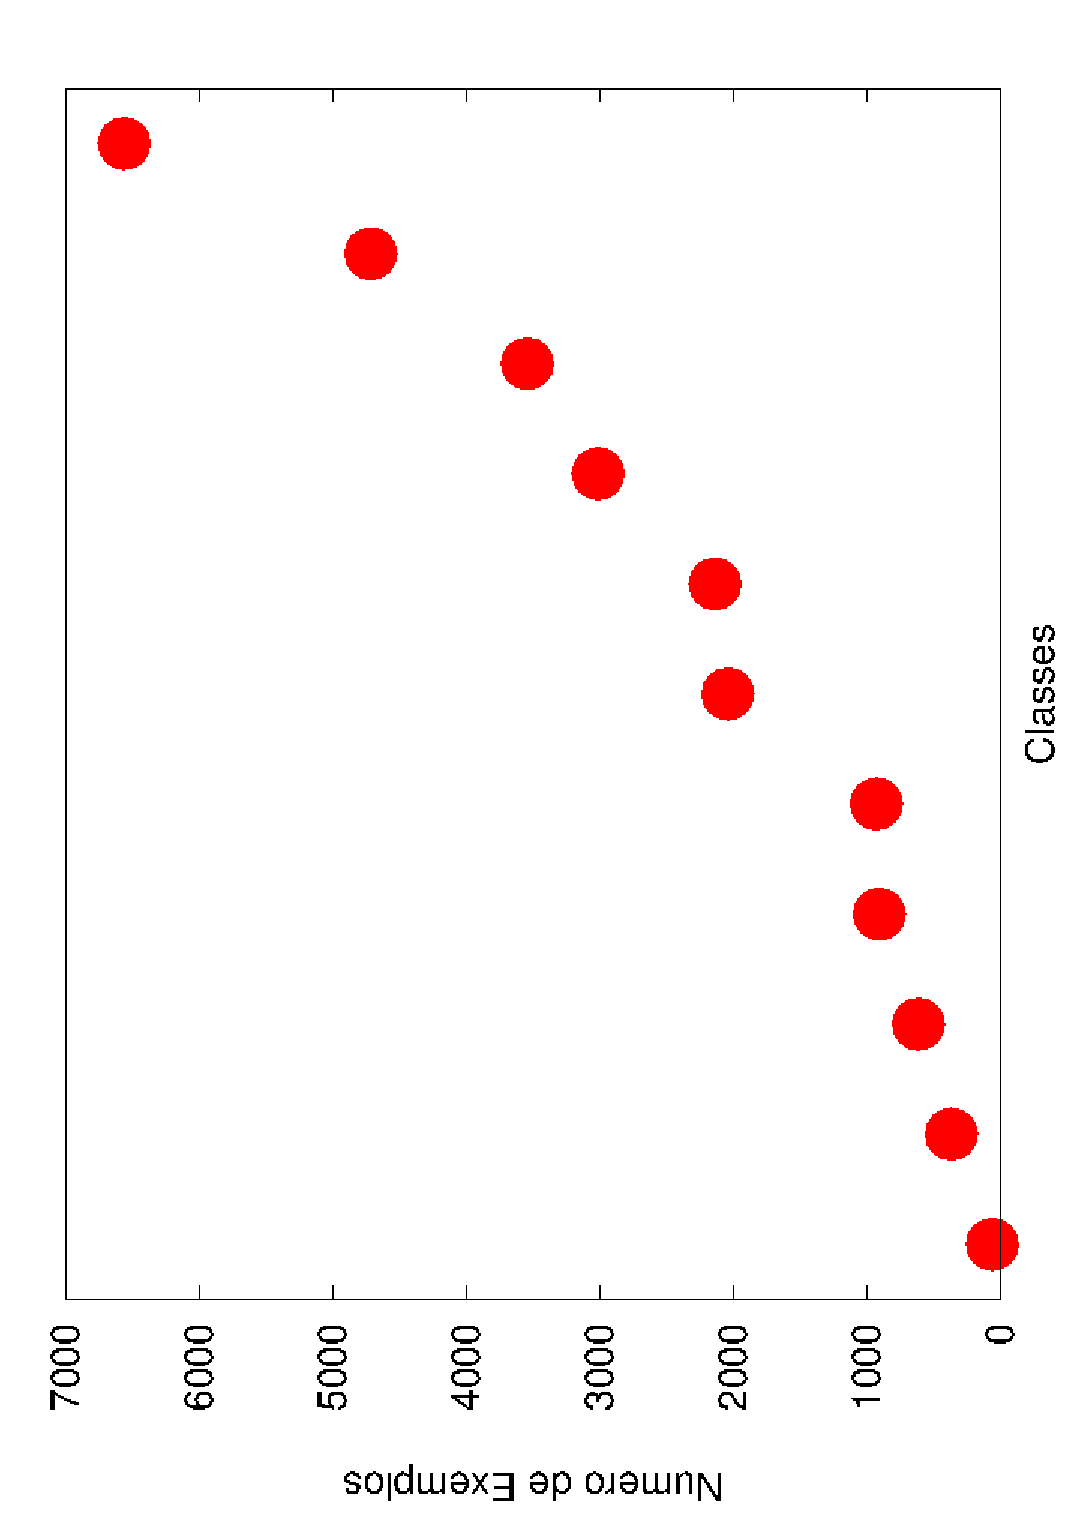
\includegraphics[angle=270, width=0.30\textwidth]{Figures/acm.eps}}
  \subfigure[][Reuters]{\label{fig::reuters}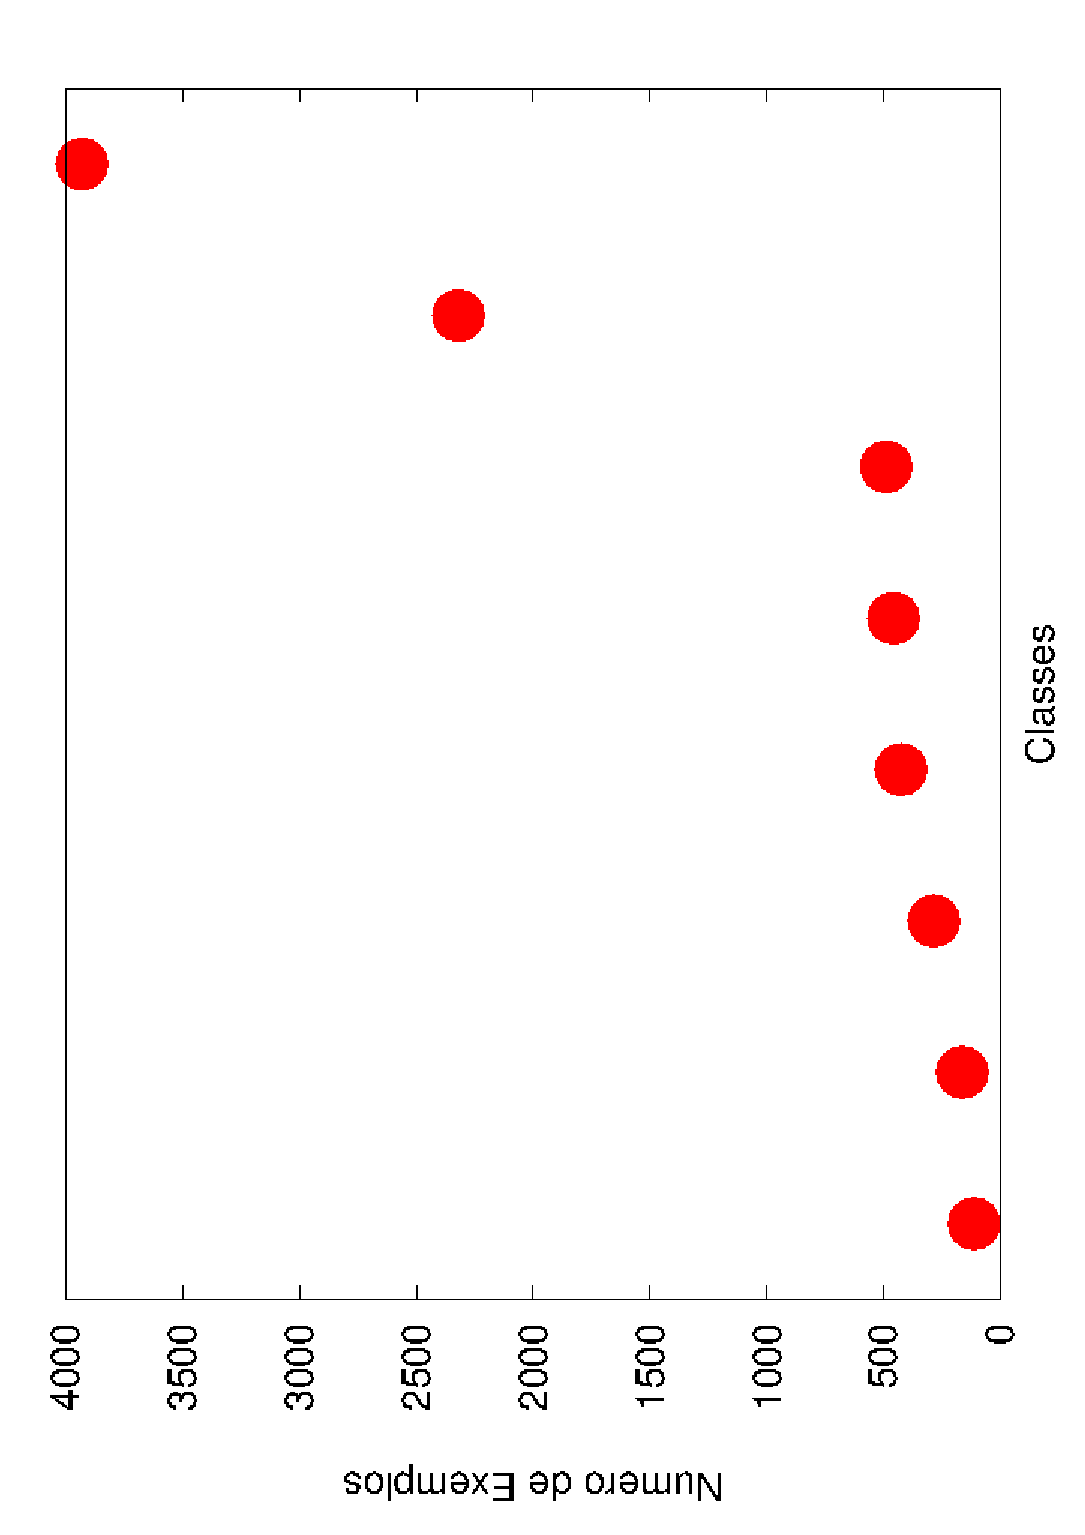
\includegraphics[angle=270, width=0.30\textwidth]{Figures/reuters.eps}}
    \\
  \subfigure[][Ohsumed]{\label{fig::ohsumed}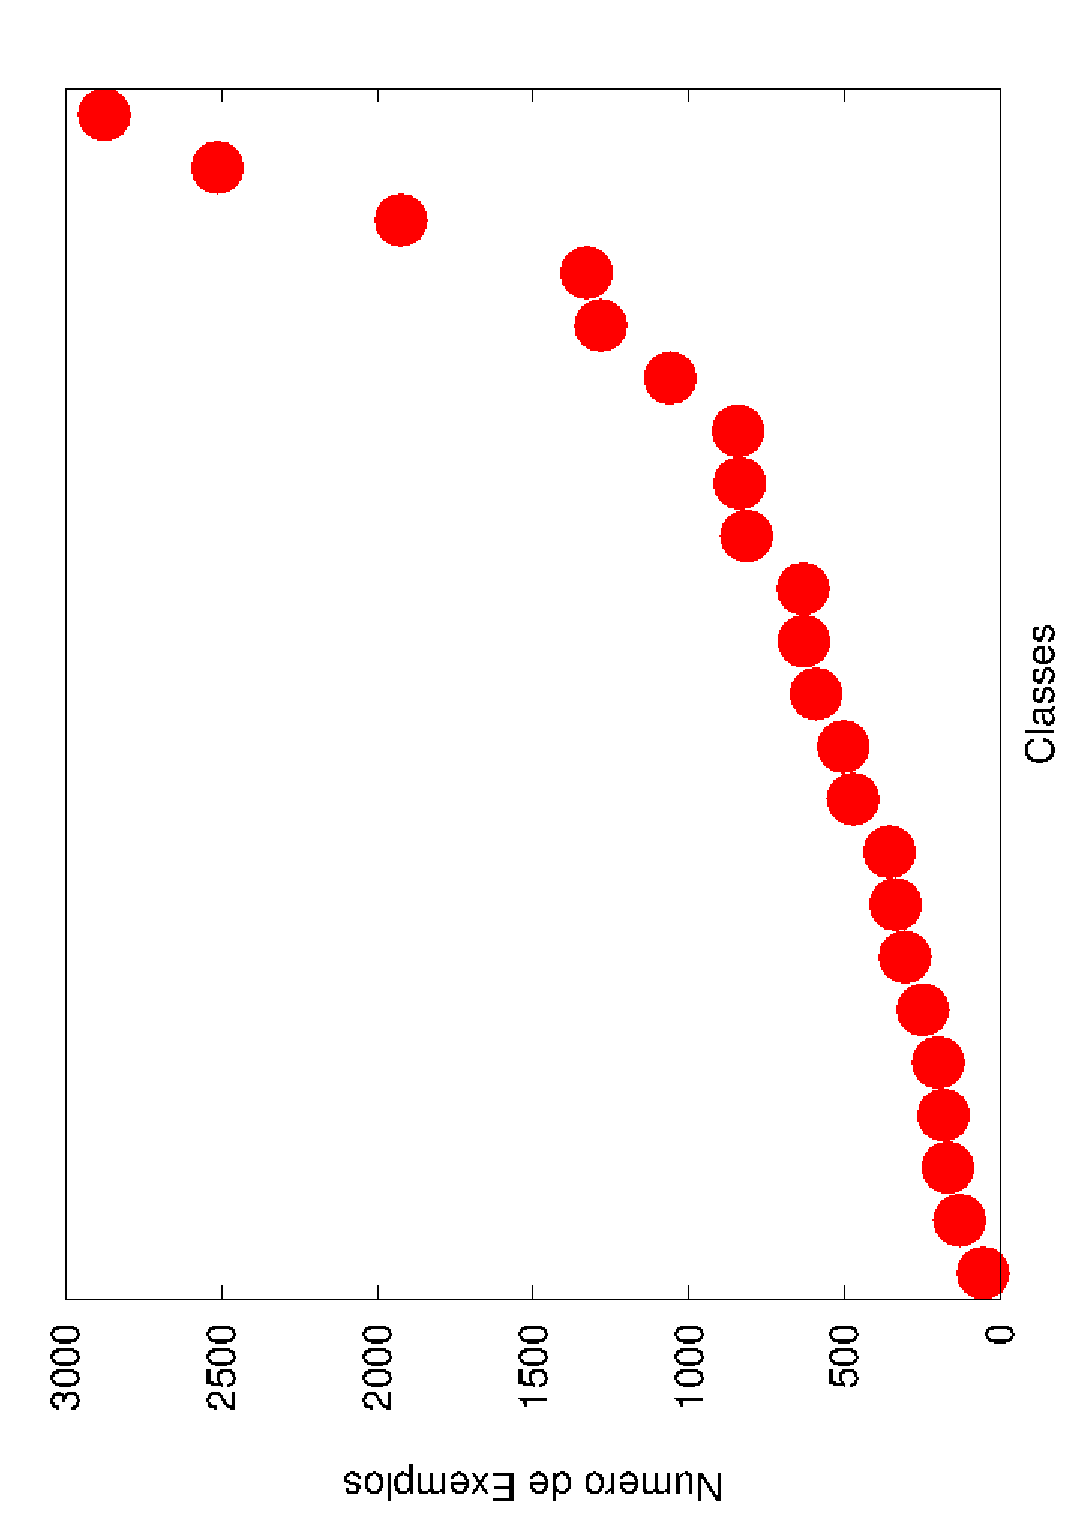
\includegraphics[angle=270, width=0.30\textwidth]{Figures/ohsumed.eps}}
  \subfigure[][20-NewsGroup]{\label{fig::20ng}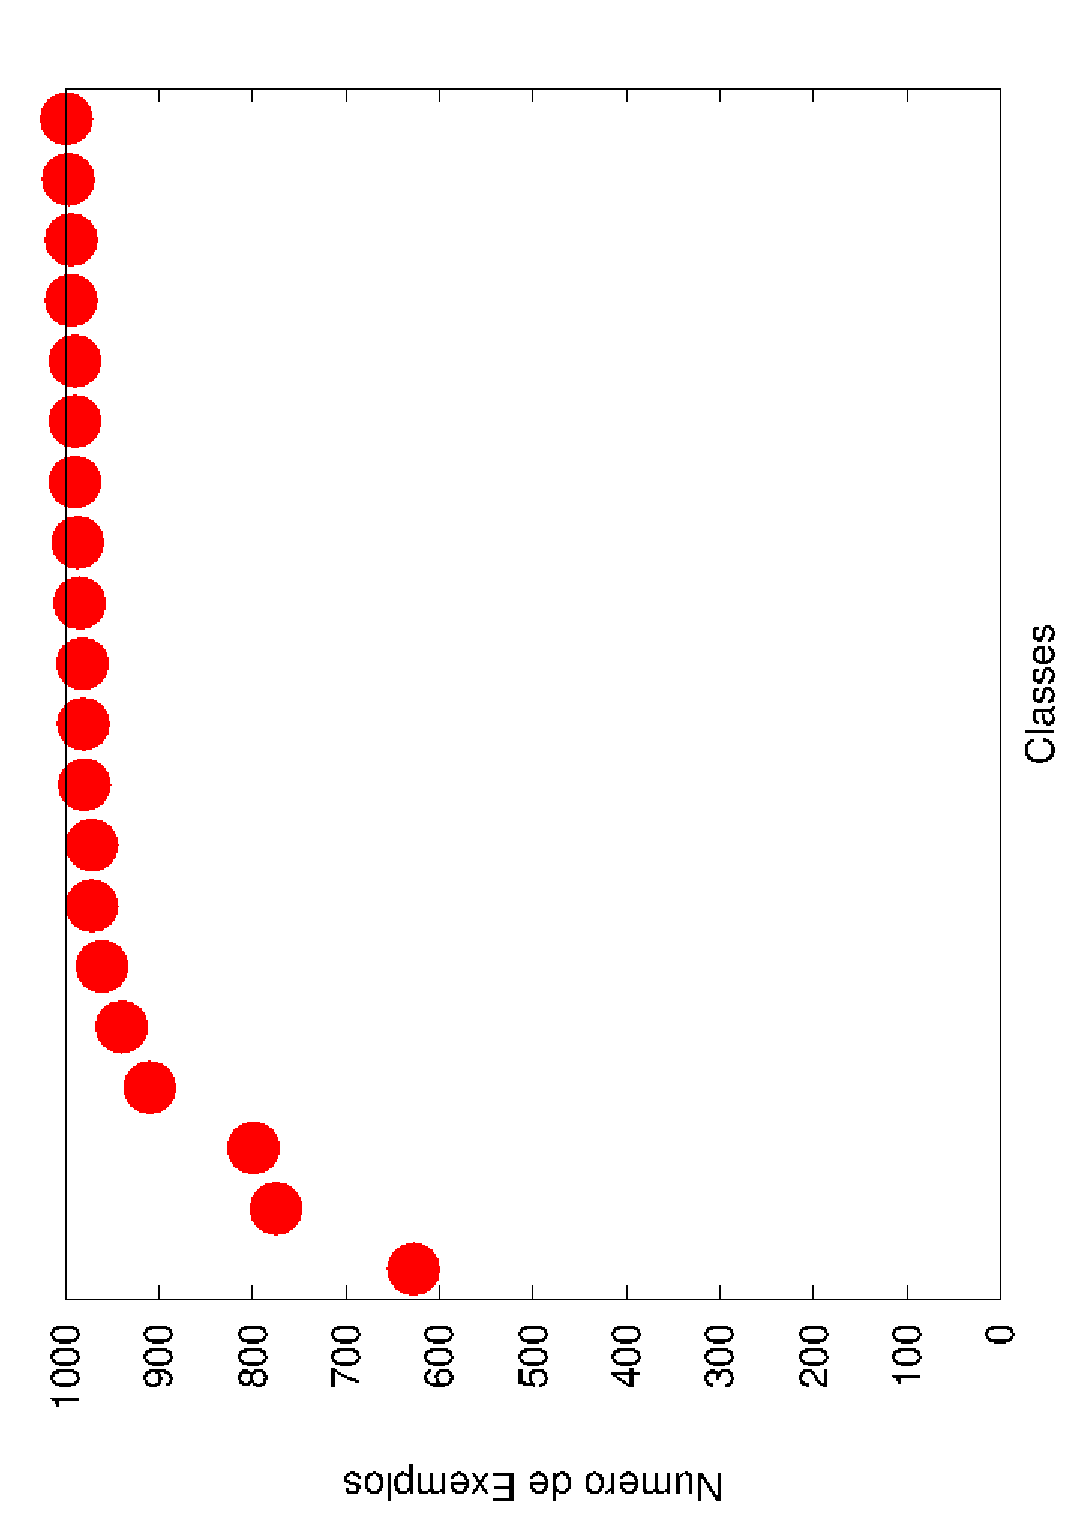
\includegraphics[angle=270, width=0.30\textwidth]{Figures/20ng.eps}}
%\caption{Distribuição dos exemplos nas classes das bases de documentos.}
%\label{fig::basesdoc}
\end{figure}

    \item Experimentos usando atributos e classificador \textit{Naïve Bayes}
    \item ACM-DL apresenta informações sobre autores e citações.
    
\end{itemize}

}


\frame{
  \frametitle{Experimentos - Credibilidade de Atributos}

\begin{table}[h]
\caption{Avaliação da Micro$F_1$ com a aplicação de diversas métricas estudadas e o \textsc{PG}.}
\tiny
\label{tab::imensamicro}
\begin{adjustwidth}{-0.95cm}{-0.95cm}% adjust the L and R margins by 1 inch
\begin{tabular}{|c||c|c|c|c|}
%\begin{tabular*}{|c|c|c|c|c|}{@{\extracolsep{\fill}}lllr}

\toprule
\textbf{Métrica} & \textbf{ACM-DL} & \textbf{20ng} & \textbf{Ohsumed} & \textbf{Reuters}\tabularnewline
\midrule
\hline
Linha de Base & 73.63 \textpm{} 2.02 & 84.94 \textpm{} 0.58 & 66.56 \textpm{} 0.66 & 93.13 \textpm{} 0.29\tabularnewline
\hline 
\rowcolor{LightCyan}
\textsc{PG} & 74.33 \textpm{} 0.72 (0.95 \ball) & 89.06 \textpm{} 0.15 (4.85 \triangOK) & 69.34 \textpm{} 0.55 (4.19 \triangOK) & 94.60 \textpm{} 0.44 (1.57 \triangOK)\tabularnewline
\hline 
DF(t) & 66.81 \textpm{} 0.64 (-9.26 \triangBAD) & 87.53 \textpm{} 0.28 (3.15 \triangOK) & 67.05 \textpm{} 0.71 (0.75 \ball) & 92.79 \textpm{} 0.77 (-0.37 \ball)\tabularnewline
\hline 
DFClasse(t,c) & 66.99 \textpm{} 0.82 (-9.02 \triangBAD) & 87.80 \textpm{} 0.31 (3.47 \triangOK) & 67.07 \textpm{} 0.55 (0.78 \ball) & 92.80 \textpm{} 0.75 (-0.35 \ball)\tabularnewline
\hline 
\rowcolor{LightCyan2}
IDF(t) & 69.60 \textpm{} 0.79 (-5.47 \triangBAD) & 86.64 \textpm{} 0.43 (2.10 \triangOK) & 60.43 \textpm{} 0.72 (-9.21 \triangBAD) & 94.29 \textpm{} 0.35 (1.25 \triangOK)\tabularnewline
\hline 
IDFClasse(t,c) & 67.07 \textpm{} 0.77 (-8.91 \triangBAD) & 21.44 \textpm{} 32.33 (-74.73 \triangBAD) & 67.28 \textpm{} 0.42 (1.09 \triangOK) & 92.74 \textpm{} 0.46 (-0.42 \ball)\tabularnewline
\hline 
TFIDF(t,c) & 72.84 \textpm{} 1.05 (-1.06 \triangBAD) & 85.04 \textpm{} 0.30 (0.21 \ball) & 66.38 \textpm{} 0.70 (-0.27 \ball) & 93.77 \textpm{} 0.36 (0.68 \triangOK)\tabularnewline
\hline 
TFICF(t,c) & 58.75 \textpm{} 1.83 (-20.20 \triangBAD) & 84.99 \textpm{} 0.31 (0.16 \ball) & 60.43 \textpm{} 0.72 (-9.21 \triangBAD) & 72.41 \textpm{} 1.73 (-22.25 \triangBAD)\tabularnewline
\hline 
MaxDom(t) & 72.25 \textpm{} 0.70 (-1.87 \triangBAD) & 85.66 \textpm{} 0.31 (0.94 \triangOK) & 67.99 \textpm{} 0.58 (2.15 \triangOK) & 92.73 \textpm{} 0.64 (-0.43 \ball)\tabularnewline
\hline 
AM(t,c) & 73.13 \textpm{} 1.05 (-0.68 \triangBAD) & 81.98 \textpm{} 0.48 (-1.96 \triangBAD) & 64.21 \textpm{} 0.60 (-3.52 \triangBAD) & 93.43 \textpm{} 0.38 (0.31 \ball)\tabularnewline
\hline 
MaxAM(t) & 72.17 \textpm{} 0.67 (-1.97 \triangBAD) & 85.36 \textpm{} 0.18 (0.59 \ball) & 67.97 \textpm{} 0.61 (2.12 \triangOK) & 92.73 \textpm{} 0.64 (-0.43 \ball)\tabularnewline
\hline 
%\rowcolor{LightCyan}
CHI(t,c) & 69.86 \textpm{} 0.74 (-5.12 \triangBAD) & 87.23 \textpm{} 0.39 (2.79 \triangOK) & 67.99 \textpm{} 0.54 (2.16 \triangOK) & 93.76 \textpm{} 0.54 (0.67 \triangOK)\tabularnewline
\hline 
DOM(t,c) & 73.38 \textpm{} 0.97 (-0.33 \triangBAD) & 84.65 \textpm{} 0.37 (-0.24 \ball) & 64.15 \textpm{} 0.59 (-3.62 \triangBAD) & 93.43 \textpm{} 0.38 (0.31 \ball)\tabularnewline
\hline 
GSS(t,c) & 69.65 \textpm{} 0.71 (-5.40 \triangBAD) & 72.19 \textpm{} 7.43 (-14.93 \triangBAD) & 67.95 \textpm{} 0.56 (2.10 \triangOK) & 93.77 \textpm{} 0.54 (0.68 \triangOK)\tabularnewline
\hline 
CE(t) & 44.65 \textpm{} 0.34 (-39.35 \triangBAD) & 54.16 \textpm{} 1.48 (-36.17 \triangBAD) & 31.86 \textpm{} 0.13 (-52.13 \triangBAD) & 76.72 \textpm{} 0.44 (-17.67 \triangBAD)\tabularnewline
\hline 
TF(t) & 66.16 \textpm{} 5.91 (-10.14 \triangBAD) & 85.44 \textpm{} 0.69 (0.68 \ball) & 64.73 \textpm{} 3.16 (-2.74 \ball) & 86.32 \textpm{} 9.91 (-7.31 \ball)\tabularnewline
\bottomrule
\end{tabular}
\end{adjustwidth}
\end{table}

\begin{itemize}
    \item Todas métricas em separado foram piores para a ACM-DL.
    \item Para as outras 3 bases, menos de 50\% das métricas foram melhores.  
\end{itemize}


}

\frame{
  \frametitle{Experimentos}

\begin{table}[h]
\caption{Avaliação da Macro$F_1$ com a aplicação de diversas métricas estudadas e o \textsc{PG}.}
\label{tab::imensamacro}
\tiny
\begin{adjustwidth}{-0.95cm}{-0.95cm}% adjust the L and R margins by 1 inch
\begin{tabular}{|c||c|c|c|c|}
\toprule
\textbf{Métricas} & \textbf{ACM-DL}& \textbf{20ng}& \textbf{Ohsumed}& \textbf{Reuters}\tabularnewline
\midrule
\hline
Linha de Base& 57.26 \textpm{} 2.08& 83.68 \textpm{} 0.82& 54.76 \textpm{} 1.27& 81.96 \textpm{} 1.44\tabularnewline
\hline 
\rowcolor{LightCyan}
\textsc{PG}& 59.72 \textpm{} 1.26 (4.30 \triangOK)& 88.69 \textpm{} 0.22 (5.99 \triangOK)& 63.56 \textpm{} 0.89 (16.06 \triangOK)& 89.33 \textpm{} 0.90 (8.99 \triangOK)\tabularnewline
\hline 
DF(t)& 55.83 \textpm{} 0.57 (-2.50 \triangBAD)& 86.85 \textpm{} 0.39 (3.86 \triangOK)& 61.43 \textpm{} 1.49 (12.18 \triangOK)& 87.24 \textpm{} 0.98 (6.44 \triangOK)\tabularnewline
\hline 
DFClasse(t,c)& 55.60 \textpm{} 0.70 (-2.89 \triangBAD) & 87.22 \textpm{} 0.38 (4.30 \triangOK)& 61.71 \textpm{} 1.41 (12.69 \triangOK)& 87.56 \textpm{} 1.55 (6.84 \triangOK) \tabularnewline
\hline 
IDF(t) & 56.84 \textpm{} 0.80 (-0.73 \triangBAD) & 85.58 \textpm{} 0.57 (2.35 \triangOK) & 57.07 \textpm{} 0.52 (4.22 \triangOK) & 89.01 \textpm{} 0.60 (8.61 \triangOK)\tabularnewline
\hline 
IDFClasse(t,c) & 54.88 \textpm{} 0.61 (-4.15 \triangBAD) & 17.43 \textpm{} 33.83 (-79.16 \triangBAD) & 61.50 \textpm{} 1.36 (12.31 \triangOK) & 85.94 \textpm{} 0.85 (4.86 \triangOK) \tabularnewline
\hline 
TFIDF(t,c)& 58.33 \textpm{} 1.08 (1.87 \triangOK)& 83.85 \textpm{} 0.40 (0.28 \ball)& 56.37 \textpm{} 1.29 (2.94 \triangOK)& 85.25 \textpm{} 0.64 (4.01 \triangOK)\tabularnewline
\hline 
TFICF(t,c)& 50.63 \textpm{} 0.97 (-11.58 \triangBAD)& 80.60 \textpm{} 1.52 (-3.61 \triangBAD)& 57.07 \textpm{} 0.52 (4.22 \triangOK)& 66.44 \textpm{} 1.50 (-18.93 \triangBAD)\tabularnewline
\hline 
MaxDom(t)& 58.74 \textpm{} 1.27 (2.58 \triangOK)& 84.31 \textpm{} 0.52 (0.82 \ball)& 62.60 \textpm{} 0.83 (14.32 \triangOK)& 87.07 \textpm{} 0.95 (6.23 \triangOK)\tabularnewline
\hline 
\rowcolor{LightCyan2}
AM(t,c)& 58.02 \textpm{} 1.73 (1.33 \ball)& 83.78 \textpm{} 0.27 (-1.27 \triangBAD) & 52.21 \textpm{} 1.12 (-4.65 \triangBAD)& 85.28 \textpm{} 0.87 (4.06 \triangOK)\tabularnewline
\hline 
MaxAM(t)& 58.64 \textpm{} 1.20 (2.41 \triangOK)& 83.68 \textpm{} 0.27 (0.07 \ball)& 62.93 \textpm{} 1.03 (14.91 \triangOK)& 87.07 \textpm{} 0.95 (6.23 \triangOK)\tabularnewline
\hline 
%\rowcolor{LightCyan}
CHI(t,c)& 56.81 \textpm{} 1.00 (-0.78 \ball)& 86.54 \textpm{} 0.46 (3.49 \triangOK)& 62.59 \textpm{} 1.41 (14.30 \triangOK)& 88.31 \textpm{} 0.95 (7.75 \triangOK)\tabularnewline
\hline 
DOM(t,c)& 58.34 \textpm{} 1.62 (1.89 \ball)&  83.21 \textpm{} 0.55 (-0.49 \triangBAD)& 51.77 \textpm{} 1.00 (-5.47 \triangBAD)& 85.28 \textpm{} 0.87 (4.06 \triangOK)\tabularnewline
\hline 
GSS(t,c)& 56.90 \textpm{} 0.91 (-0.62 \ball)& 74.52 \textpm{} 5.89 (-10.89 \triangBAD)& 62.57 \textpm{} 1.39 (14.25 \triangOK)& 88.43 \textpm{} 0.91 (7.90 \triangOK)\tabularnewline
\hline 
CE(t)& 22.94 \textpm{} 0.41 (-59.93 \triangBAD)&  50.23 \textpm{} 1.40 (-39.93 \triangBAD)& 8.78 \textpm{} 0.11 (-83.96 \triangBAD)& 31.55 \textpm{} 1.48 (-61.73 \triangBAD)\tabularnewline
\hline 
TF(t)& 54.89 \textpm{} 3.33 (-4.14 \ball)& 83.12 \textpm{} 2.08 (-0.59 \ball)& 58.48 \textpm{} 2.76 (6.80 \triangOK)& 79.64 \textpm{} 9.43 (-2.83 \ball)\tabularnewline
\bottomrule
\end{tabular}
\end{adjustwidth}
%\end{scriptsize}
\end{table}

%\end{tabularx}}

\begin{itemize}
    \item Reuters e Ohsumed, por serem as mais desbalanceadas, foram as bases que obtiveram melhores resultados (mais de 50\% das métricas isoladas obtêm melhorias).
\end{itemize}

}

\frame{
  \frametitle{Experimentos}

\begin{table}[!h]
\renewcommand{\arraystretch}{1.3}
\centering
\caption{Funções de credibilidade geradas para cada uma das bases. Selecionadas entre as 5 evoluídas.}
\label{tab::representantes}
\small
\begin{tabular}{|c||c|}
\toprule
\textbf{Base} & \textbf{Função de Credibilidade}\tabularnewline
\midrule
\hline
ACM-DL   & $F_{ACM-DL} =  DOM^{(GSS)^{(CE + TF)}} $\tabularnewline
\hline 
20ng & $F_{20ng} = DF + MaxAM + (\dfrac{ CHI } { TFIDF^{(MaxTFIDF)} }) $\tabularnewline
\hline 
Ohsumed  & $ F_{Ohsumed} = (\dfrac{AM}{MaxIG \times CC^{(sumDF)}} )^{(TFICF)^{(TFICF)}} $\tabularnewline
\hline 
Reuters & $ F_{Reuters} = IG^{(MaxIG \times GINI)}$\tabularnewline
\bottomrule
\end{tabular}
\end{table}

}


\frame{

\frametitle{Experimentos - Avaliação de Generalidade}

\vspace{-0.5cm}

\begin{table}[!h]
\centering
\caption{Micro$F_1$ obtida pelo \textit{Naïve Bayes} ao usar a função de credibilidade $F_{base}$ gerada uma dada base nas demais.}
\vspace{-0.5cm}
\label{tab::generalizacao-Micro}
\tiny
\begin{adjustwidth}{-0.7cm}{-0.7cm}% adjust the L and R margins by 1 inch
\begin{tabular}{|c|c|c|c|c|}
\toprule
 & \textbf{ACM-DL} & \textbf{20ng} & \textbf{Ohsumed} & \textbf{Reuters}\tabularnewline
\midrule
\hline
Linha de Base & 73.63 \textpm{} 0.90 & 84.86 \textpm{} 0.54 & 66.56 \textpm{} 0.66 & 93.13 \textpm{} 0.29\tabularnewline
\hline 
$F_{ACM-DL}$ & 75.04 \textpm{} 0.88 (1.91 \triangOK) & 84.45 \textpm{} 0.35 (-0.49 \triangBAD) & 66.06 \textpm{} 0.59 (-0.75 \ball) & 92.68 \textpm{} 0.45 (-0.48 \triangBAD)\tabularnewline
\hline 
$F_{20ng}$ & 66.69 \textpm{} 0.65 (-9.42 \triangBAD) & 88.97 \textpm{} 0.17 (4.84 \triangOK) & 67.94 \textpm{} 0.62 (2.08 \triangOK)  & 94.01 \textpm{} 0.53 (0.94 \triangOK)\tabularnewline
\hline 
$F_{Ohsumed}$ & 70.09 \textpm{} 0.82 (-4.81 \triangBAD) & 85.60 \textpm{} 0.27 (0.87 \triangOK) & 69.54 \textpm{} 0.69 (4.49 \triangOK) & 93.45 \textpm{} 0.57 (0.34 \ball)\tabularnewline
\hline 
$F_{Reuters}$ & 66.55 \textpm{} 0.89 (-9.61 \triangBAD) & 87.04 \textpm{} 0.41 (2.57 \triangOK) & 63.32 \textpm{} 0.82 (-4.86 \triangBAD) & 94.87 \textpm{} 0.25 (1.86 \triangOK)\tabularnewline
\bottomrule
\end{tabular}
\end{adjustwidth}
\end{table}

\vspace{-0.5cm}

\begin{table}[!h]
\centering
\caption{Macro$F_1$ obtida pelo \textit{Naïve Bayes} ao usar a função de credibilidade $F_{base}$ gerada uma dada base nas demais.}
\vspace{-0.5cm}
\label{tab::generalizacao-Macro}
\tiny
\begin{adjustwidth}{-0.7cm}{-0.7cm}% adjust the L and R margins by 1 inch
\begin{tabular}{|c|c|c|c|c|}
\toprule
 & \textbf{ACM-DL} & \textbf{20ng} & \textbf{Ohsumed} & \textbf{Reuters}\tabularnewline
\midrule
\hline
Linha de Base & 57.26 \textpm{} 0.93 & 83.62 \textpm{} 0.74 & 54.76 \textpm{} 1.27 & 81.96 \textpm{} 1.44\tabularnewline
\hline 
$F_{ACM-DL}$ & 60.13 \textpm{} 1.44 (5.02 \triangOK) & 82.88 \textpm{} 0.51 (-0.89 \triangBAD) & 56.41 \textpm{}  0.92 (3.00 \triangOK) & 85.49 \textpm{} 0.94 (4.31 \triangOK)\tabularnewline
\hline 
$F_{20ng}$ & 55.83 \textpm{} 0.66 (-2.50 \triangBAD) & 88.63 \textpm{} 0.18 (5.99 \triangOK) & 62.12 \textpm{} 1.41 (13.43 \triangOK) & 88.64 \textpm{} 1.03 (8.16 \triangOK)\tabularnewline
\hline 
$F_{Ohsumed}$ & 57.59 \textpm{} 0.56 (0.58 \ball) & 84.26 \textpm{}  0.49 (0.77 \triangOK) & 64.35 \textpm{} 1.17 (17.51 \triangOK) & 87.41 \textpm{} 0.64 (6.65 \triangOK)\tabularnewline
\hline 
$F_{Reuters}$ & 54.84 \textpm{} 1.44 (-4.23 \triangBAD) & 83.15 \textpm{} 2.04 (-0.56 \ball) & 57.97 \textpm{} 1.59 (5.85 \triangOK) & 89.45 \textpm{}  0.74 (9.14 \triangOK)\tabularnewline
\bottomrule 
\end{tabular}
\end{adjustwidth}
\end{table}

\begin{itemize}
\item Generaliza bem para a própria base.
\item Excluindo as funções da base da ACM-DL, as outras generalizam bem, especialmente para Macro$F_1$.
\end{itemize}

}

\frame{

    \frametitle{Experimentos - Atributos \textbf{e} Relacionamentos}

\begin{table}[!h]
\centering
\caption{Resultados do uso de credibilidade na base da \textsc{ACM-DL} explorando a credibilidade de termos, autoria e citação.}
\label{tab::fatores}
\small
\begin{adjustwidth}{-0.7cm}{-0.7cm}% adjust the L and R margins by 1 inch
\begin{tabular}{|c|c|c||c|c|}
\toprule
\multicolumn{3}{|c||}{\textbf{Fatores}} & \multirow{2}{*}{\textbf{Micro$F_1$}} & \multirow{2}{*}{\textbf{Macro$F_1$}} \tabularnewline \cline{1-3}
\textbf{Termos} & \textbf{Autoria} & \textbf{Citação} & & \multicolumn{1}{c|}{}  \tabularnewline % & \textbf{Micro$F_1$} & \textbf{Macro$F_1$}\tabularnewline
\midrule
\hline
\multicolumn{3}{|c||}{Linha de Base} & 73.63 \textpm{} 0.91 & 57.26 \textpm{} 0.93\tabularnewline
\hline 
\rowcolor{LightCyan}
X &  &  & 74.33 \textpm{} 0.72 (0.95 \ball) & 59.72 \textpm{} 1.26 (4.30 \triangOK)\tabularnewline
\hline 
\rowcolor{LightCyan}
& X &  & 76.19 \textpm{} 0.82 (3.48 \triangOK) & 60.37 \textpm{} 0.70 (5.43 \triangOK)\tabularnewline
\hline 
 &  & X & 75.58 \textpm{} 0.85 (2.65 \triangOK) & 59.00 \textpm{} 0.90 (3.04 \triangOK)\tabularnewline
\hline 
\rowcolor{LightCyan}
X & X &  & 76.70 \textpm{} 1.08 (4.18 \triangOK) & 61.82 \textpm{} 1.38 (7.96 \triangOK)\tabularnewline
\hline 
X &  & X & 75.63 \textpm{} 1.03 (2.72 \triangOK) & 60.69 \textpm{} 1.30 (5.98 \triangOK)\tabularnewline
\hline 
 & X & X & 77.29 \textpm{} 0.79 (\cred{4.98} \triangOK) & 61.41 \textpm{} 0.65 (7.25 \triangOK)\tabularnewline
\hline 
X & X & X & 77.01 \textpm{} 0.98 (\cred{4.60} \triangOK) & 62.24 \textpm{} 1.01 (8.70 \triangOK)\tabularnewline
\bottomrule
\end{tabular}
\end{adjustwidth}
\end{table}

\begin{itemize}
\item Usar mais de um fator trouxe ganhos progressivamente.
\item Única excessão é a Micro-$F_1$ ao utilizar todos os fatores: parâmetros.
\end{itemize}

}

\subsection{Bases de Atributos Categóricos}

\frame{
\frametitle{Experimentos - Bases com atributos categóricos}

\begin{figure}[h]
  \centering
  \subfigure[][cars]{\label{fig::cars}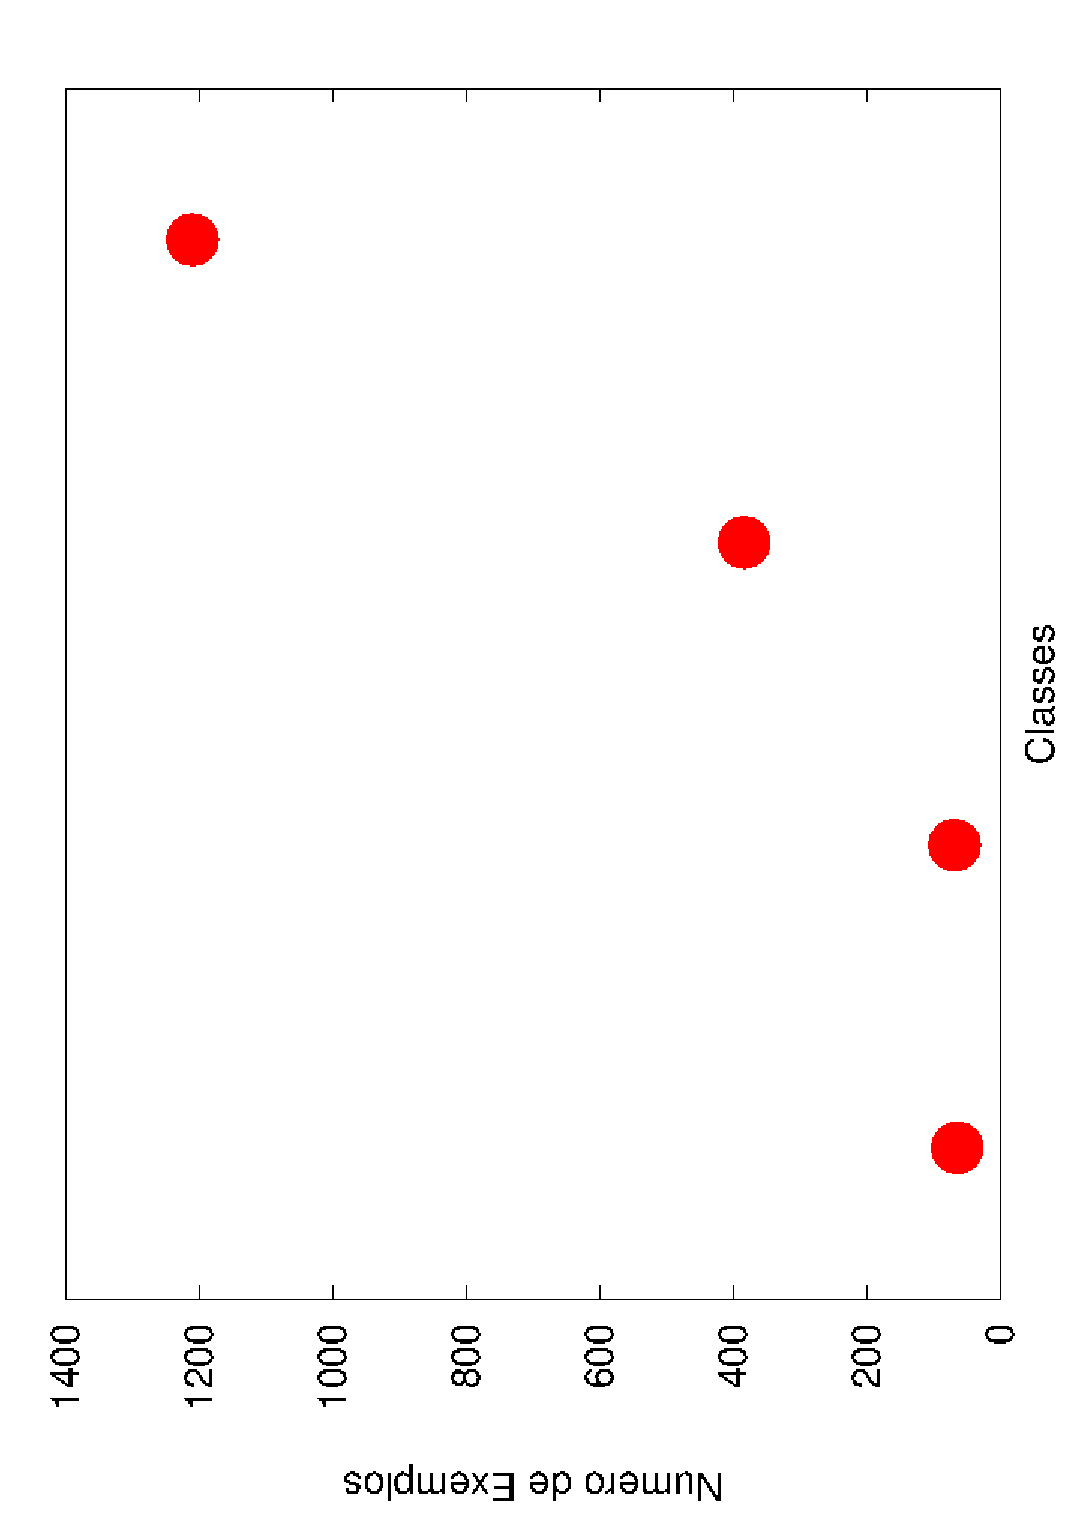
\includegraphics[angle=270, width=0.30\textwidth]{Figures/cars.eps}}
  \subfigure[][chess]{\label{fig::chess}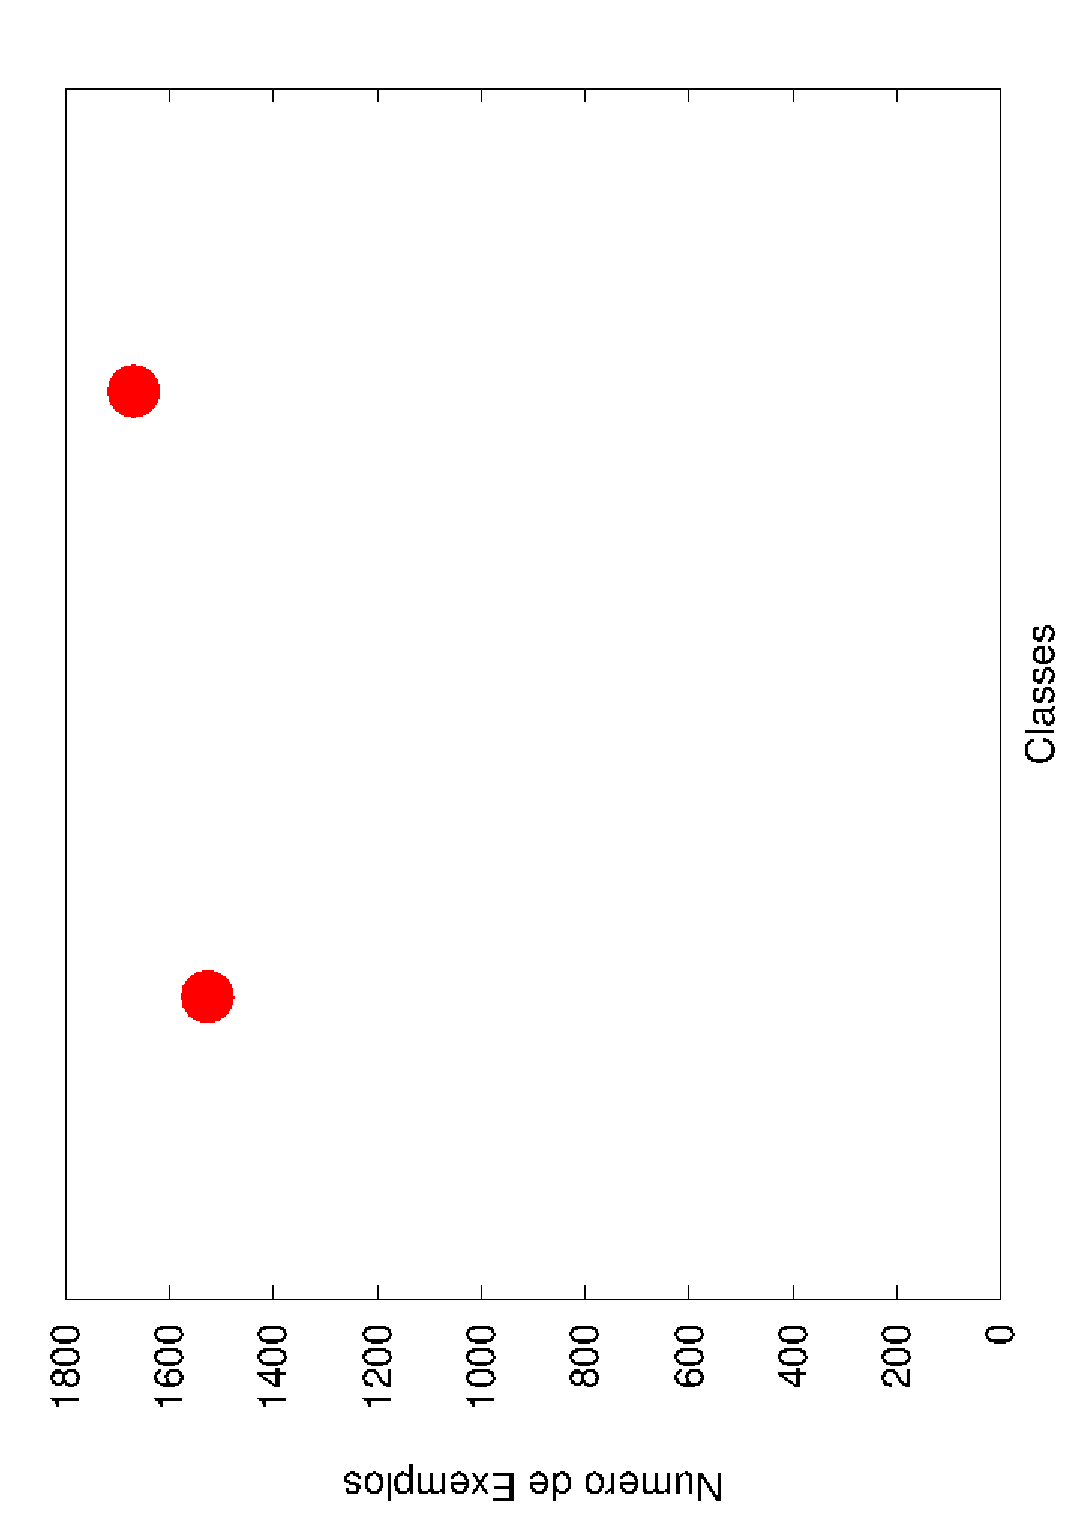
\includegraphics[angle=270, width=0.30\textwidth]{Figures/chess.eps}}
    \\
  \subfigure[][nursery]{\label{fig::nursery}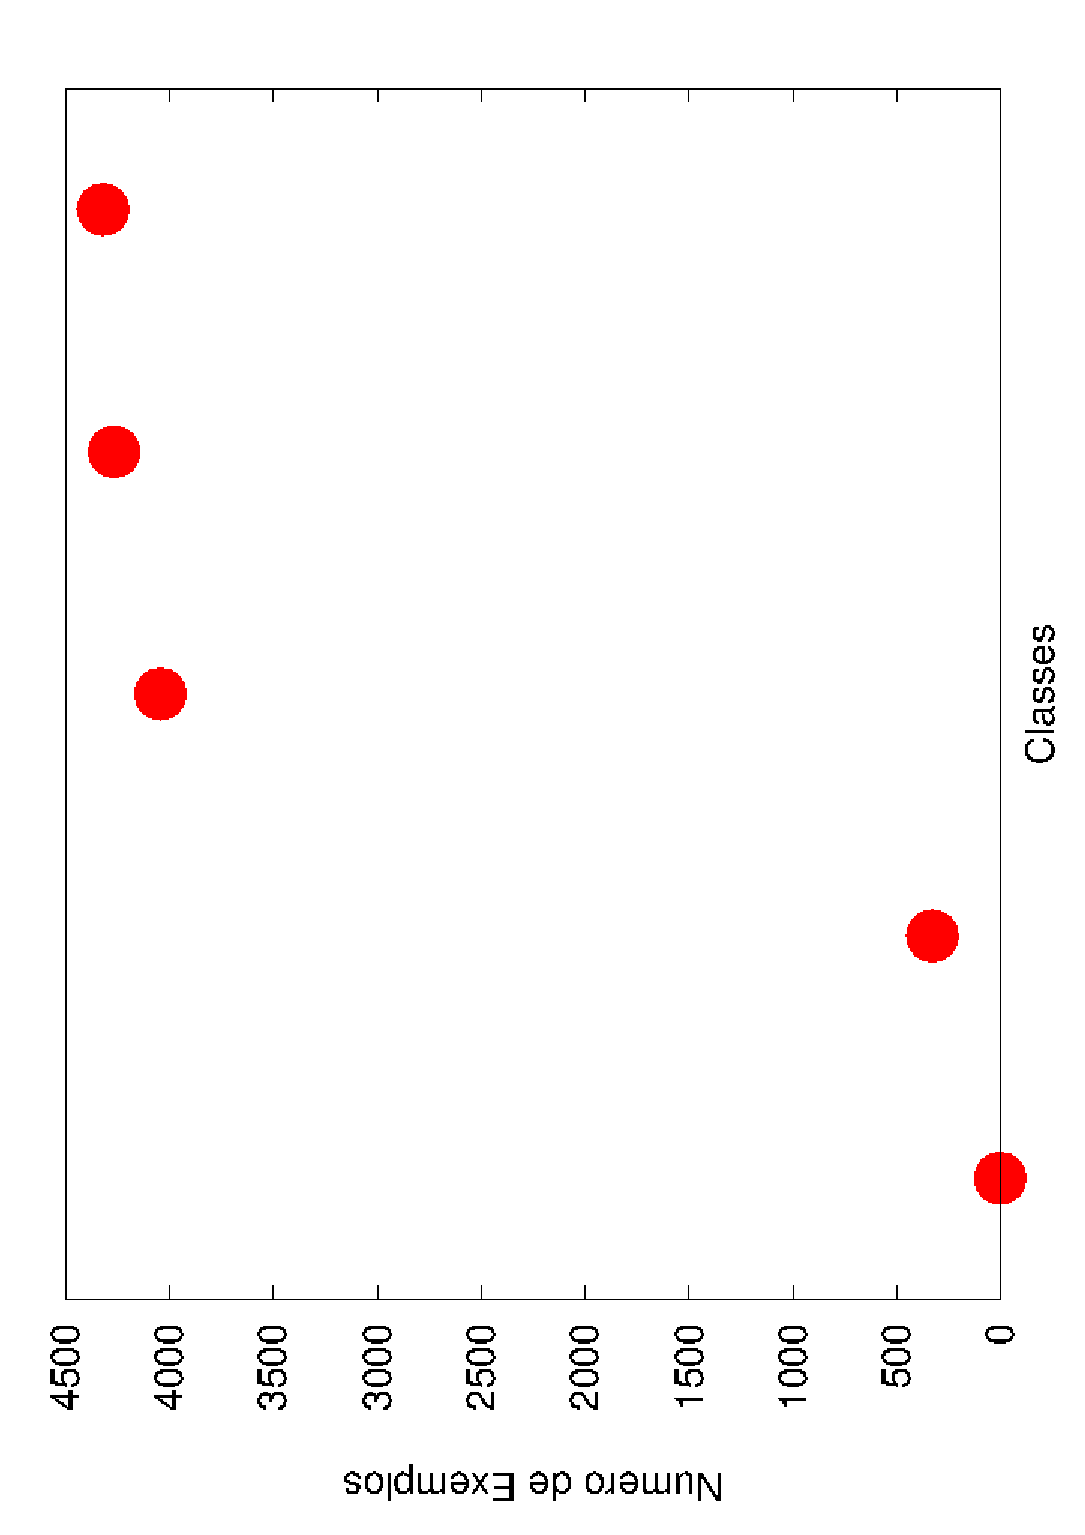
\includegraphics[angle=270, width=0.30\textwidth]{Figures/nursery.eps}}
  \subfigure[][tictactoe]{\label{fig::tictactoe}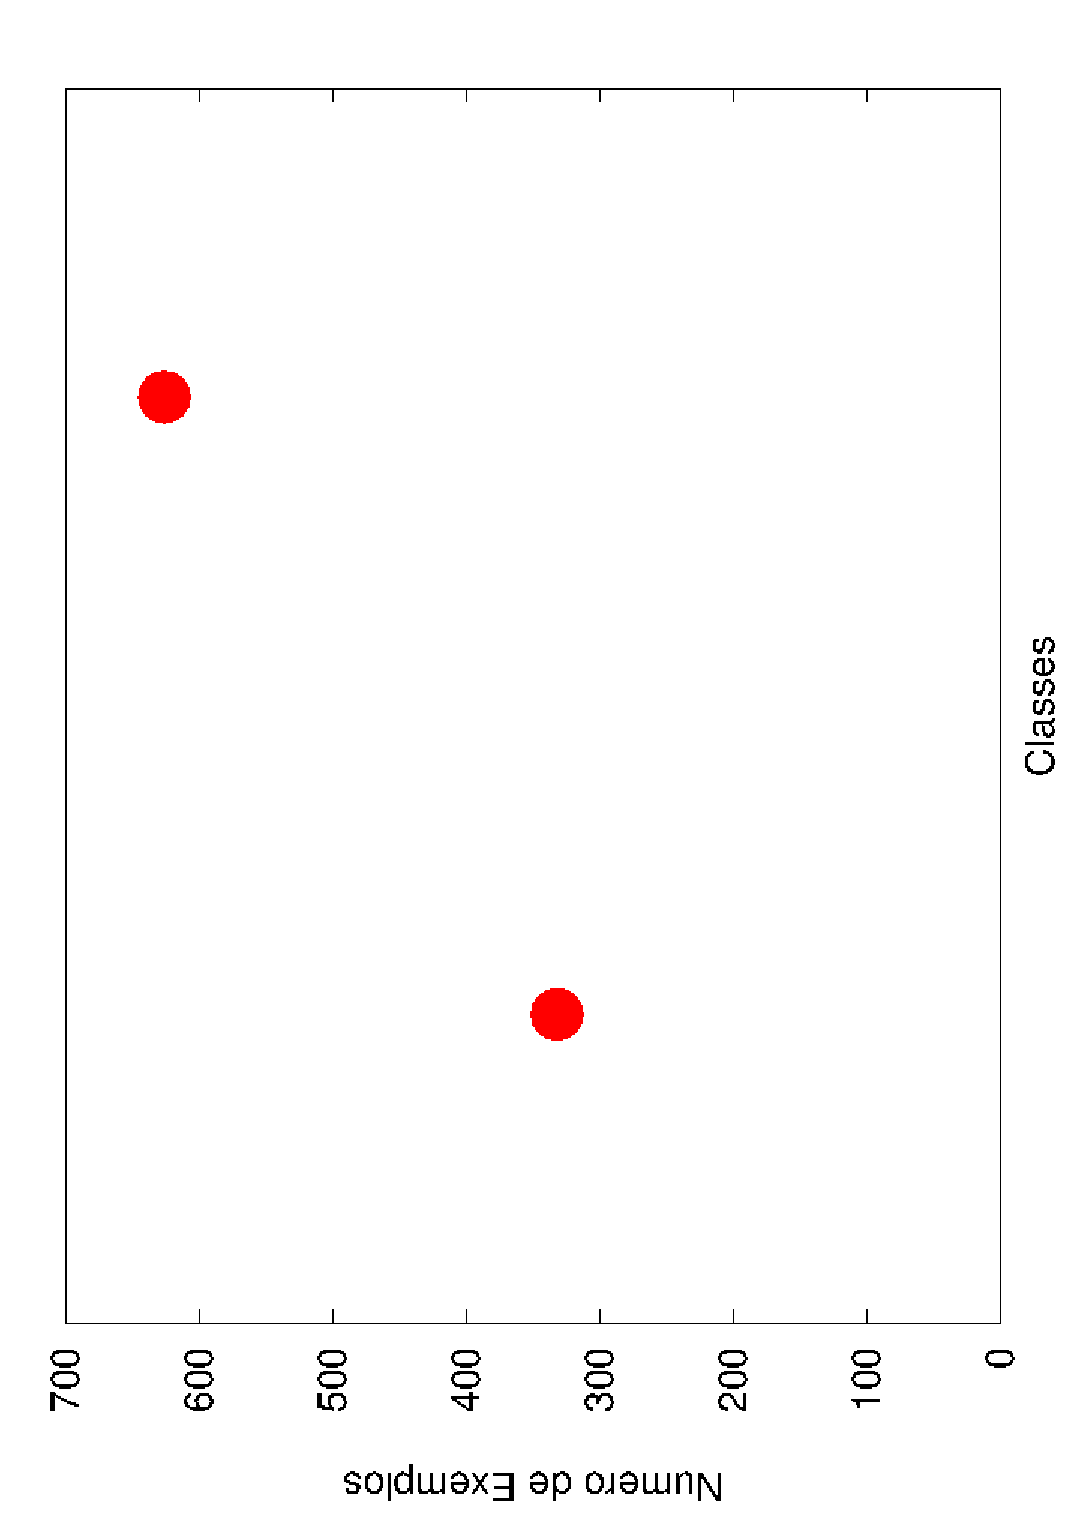
\includegraphics[angle=270, width=0.30\textwidth]{Figures/tictactoe.eps}}
\end{figure}

\begin{itemize}
\item Bases mais simples provenientes da \textsc{UCI}.
\item Experimentos usando \textsc{KNN} e \textit{Naïve Bayes}.
\item Categóricos: carro (novo, velho, semi-novo).
\end{itemize}

}




\frame{

    \frametitle{Experimentos - Atributos Categóricos}

\begin{table}[h!]
\centering
\caption{Resultados da Micro$F_1$ para as bases de atributos categóricos}
\label{tab::cat-micro}
\scriptsize
\begin{adjustwidth}{-0.3cm}{-0.3cm}% adjust the L and R margins by 1 inch
\begin{tabular}{|c||c|c|c|c|}
\toprule
\multirow{2}{*}{\textbf{Bases}} & \multicolumn{2}{c|}{\textbf{Naïve Bayes}} & \multicolumn{2}{c|}{\textbf{KNN}}\tabularnewline
\cline{2-5} 
 & \textbf{Linha de Base} & \textbf{Micro$F_1$} & \textbf{Linha de Base} & \textbf{Micro$F_1$}\tabularnewline
\midrule
\hline
\textit{Cars} & 86.32 \textpm{} 1.85 & 87.64 \textpm{} 2.53 (1.52 \triangOK) & 91.84 \textpm{} 1.95 & 92.43 \textpm{} 1.68 (0.64 \ball)\tabularnewline
\hline 
\textit{TicTacToe} & 70.63 \textpm{} 2.10 & 71.74 \textpm{} 2.02 (1.58 \triangOK) & 96.45 \textpm{} 0.85  & 97.42 \textpm{} 0.94 (1.00 \ball)\tabularnewline
\hline 
\textit{Nursery} & 90.29 \textpm{} 0.56 & 91.21 \textpm{} 0.92 (1.01 \ball) & 95.84 \textpm{} 0.73 & 96.00 \textpm{} 0.69 (0.17 \ball) \tabularnewline
\hline 
\textit{Chess} & 87.85 \textpm{} 0.69 & 88.04 \textpm{} 0.75 (0.21 \ball) & 94.77 \textpm{} 0.41  & 96.00 \textpm{} 0.60 (1.29 \triangOK)\tabularnewline
\bottomrule
\end{tabular}
\end{adjustwidth}
\end{table}

\begin{table}[h!]
\centering
\caption{Resultados da Macro$F_1$ para as bases de atributos categóricos}
\label{tab::cat-macro}
\scriptsize
\begin{adjustwidth}{-0.5cm}{-0.5cm}
\begin{tabular}{|c||c|c|c|c|}
\toprule
\multirow{2}{*}{\textbf{Bases}} & \multicolumn{2}{c|}{\textbf{Naïve Bayes}} & \multicolumn{2}{c|}{\textbf{KNN}}\tabularnewline
\cline{2-5} 
 & \textbf{Linha de Base} & \textbf{Macro$F_1$} & \textbf{Linha de Base} & \textbf{Macro$F_1$}\tabularnewline
\midrule
\hline
\textit{Cars} & 67.74 \textpm{} 3.08 & 76.85 \textpm{} 5.65 (\cred{13.44} \triangOK) & 75.36 \textpm{} 3.44 & 81.77 \textpm{} 3.90 (\cred{8.51} \triangOK)\tabularnewline
\hline 
\textit{TicTacToe} & 64.48 \textpm{} 2.12 & 64.10 \textpm{} 1.96 (-0.59 \ball) & 95.99 \textpm{} 0.98 & 97.12 \textpm{} 1.10 (1.18 \ball)\tabularnewline
\hline 
\textit{Nursery} & 66.19 \textpm{} 7.41 & 77.19 \textpm{} 12.80 (\cred{16.62} \triangOK) & 80.83 \textpm{} 9.06  &	84.46 \textpm{} 9.22 (\cred{4.50}\triangOK) \tabularnewline
\hline 
\textit{Chess} & 87.81 \textpm{} 0.68 & 88.03 \textpm{} 0.75 (0.25 \ball) & 94.75 \textpm{} 0.40  & 95.98 \textpm{} 0.61 (1.30 \triangOK)\tabularnewline
\bottomrule
\end{tabular}
\end{adjustwidth}
\end{table}

}

\subsection{Base de Bioinformática}


\frame{
\frametitle{Experimentos - Bases}

\begin{figure}[h]
  \centering
  \caption{Base de Assinaturas Estruturais Proteicas}
  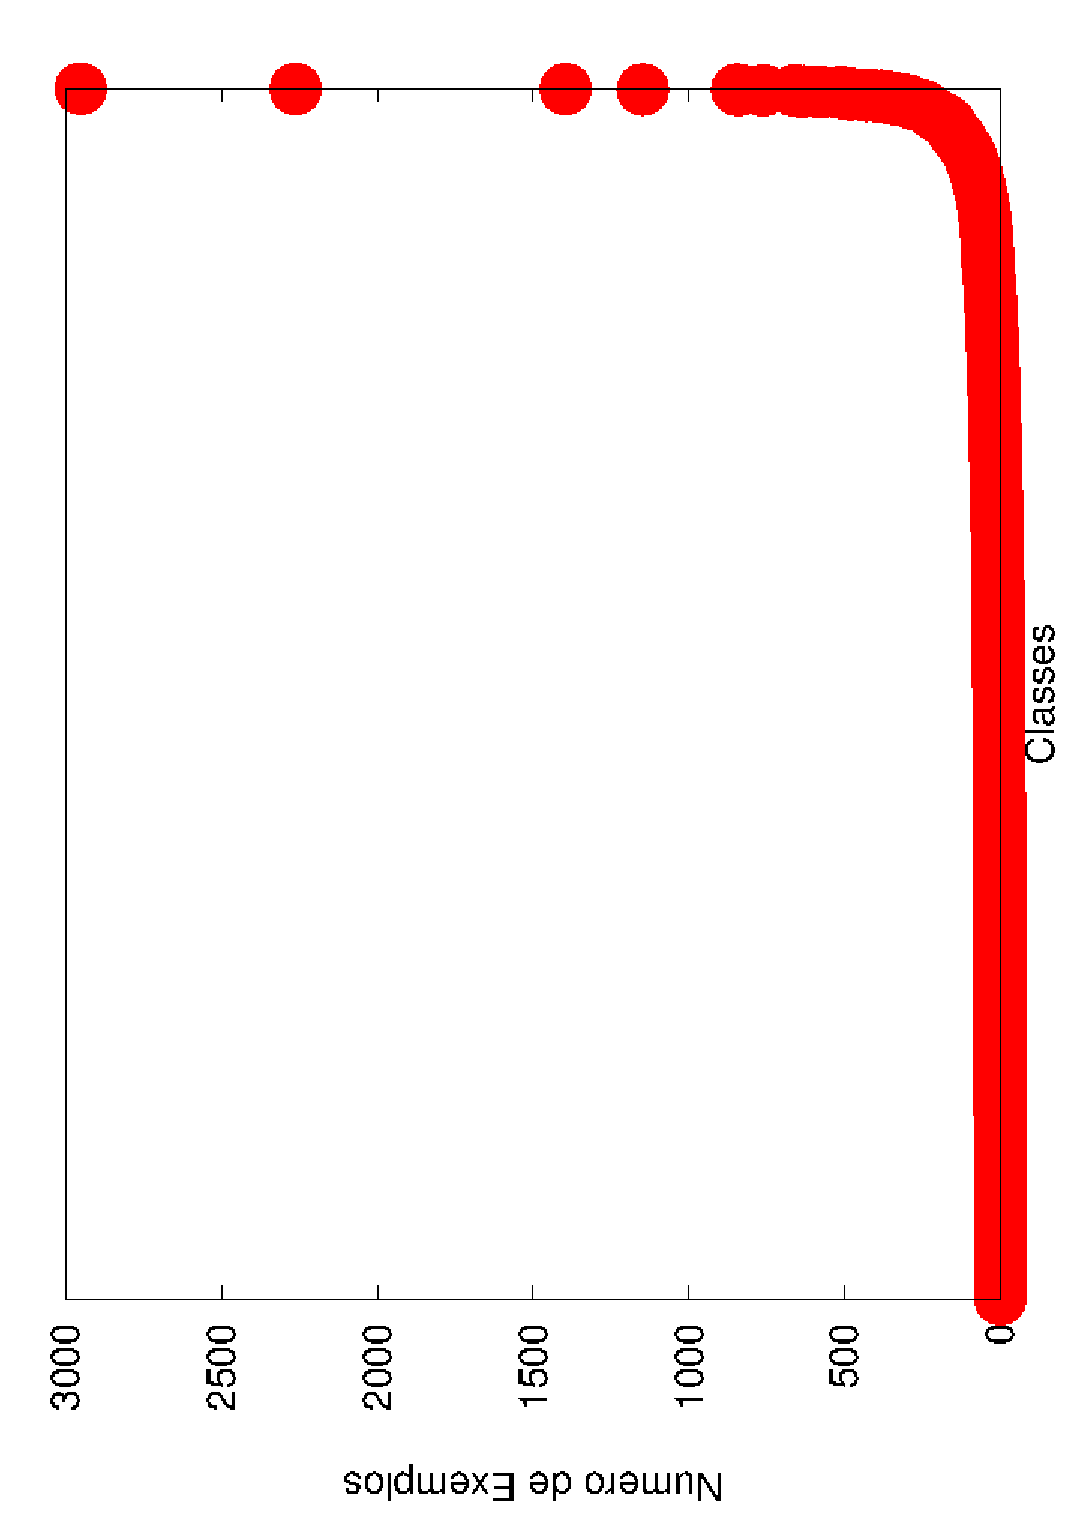
\includegraphics[angle=270, width=0.30\textwidth]{Figures/astral.eps}
\end{figure}

\begin{itemize}
\item Atributos numéricos: não temos a credibilidade definida.
\item Exploramos os relacionamentos entre as proteínas baseado em uma rede de simalaridade entre as mesmas.
\item Usado método \textsc{BLAST} para o calculo de similaridade.
\item Base muito grande: menos treinamento.
\end{itemize}

}



\frame{

\frametitle{Bioinformática}


\begin{table}[h!]
\small
%\begin{adjustwidth}{-0.1cm}{-0.1cm}% adjust the L and R margins by 1 inch
\caption{Resultados da Micro$F_1$ e Macro$F_1$ para a base de bioinformática.}
\label{tab::bioinformatica}
%\begin{footnotesize}
\begin{tabular}{|c||c|c|}
\toprule
\textbf{Algoritmo} & \textbf{Micro$F_1$} & \textbf{Macro$F_1$}\tabularnewline
\midrule
\hline 
Linha de Base & 70.23 \textpm{} 1.402 & 50.28 \textpm{} 1.44\tabularnewline
\hline 
%Vizinhos Peso Unitário & 80.37 \textpm{} 0.24 (14.33 \triangOK) & 40.28 \textpm{} 0.39 (-19.89 \triangBAD)\tabularnewline
%\hline 
Vizinhos Peso Aresta & 82.59 \textpm{} 0.26 (17.49 \triangOK)  &  43.53 \textpm{} 0.47 (-13.43 \triangBAD)\tabularnewline
\hline 
\rowcolor{LightCyan}
\textsc{PG}& 88.98 \textpm{} 4.87 (26.58 \triangOK) & 75.81 \textpm{} 4.51 (50.78 \triangOK)\tabularnewline
\bottomrule
\end{tabular}
%\end{adjustwidth}
\end{table}

\begin{itemize}
\item Linha de base: somente o \textsc{KNN}.
\item Vizinhos Peso Aresta: algoritmo simples que somente observa os vizinhos imediatos.
\item PG: \textsc{KNN} + credibilidade de relacionamentos.
\end{itemize}



}

\section{Conclusões}
\subsection{}

\frame{
  \frametitle{Conclusões}

  \begin{itemize}

    \item Utilizamos o conceito de credibilidade para diferenciar os exemplos contidos no treino.
    \vskip0.5cm
    \item Modelamos a credibilidade usando dois fatores: os \textbf{atributos} e os \textbf{relacionamentos} entre os exemplos.
    \vskip0.5cm
    \item As métricas para credibilidade dos \textbf{atributos} foram modelados através de métricas de seleção de atributos.
    \vskip0.5cm
    \item As métricas para credibilidade dos \textbf{relacionamentos} foram modelados usando métricas de Redes Complexas.
    \vskip0.5cm
 
 \end{itemize}
}

\frame{
  \frametitle{Conclusões}

  \begin{itemize}

    \item Número muito grande de métricas geradas: solução com \textbf{Programação Genética}
    \vskip0.5cm
    \item Avaliamos 9 bases de dados em 3 conjuntos de experimentos distintos e 2 algoritmos de classificação.
    \vskip0.5cm
    \item Melhorias superiores a 10\% na Micro e Macro$F_1$ em vários dos experimentos com bases textuais e categóricas.
    \vskip0.5cm
    \item Melhorias de \textbf{26\%} na Micro$F_1$ e \textbf{50\%} na Macro$F_1$ no experimento com a base de bioinformática.
    \vskip0.5cm
 
 \end{itemize}
}



\frame{
  \frametitle{Trabalho Futuro}
  \begin{itemize}
    \item Destacamos como principais trabalhos futuros:
    
    \begin{enumerate}
        \item Incorporar a credibilidade em outros classificadores: \textsc{SVM}, árvores de decisão, regras de associação, etc.
            \vskip0.25cm
        \item Testar outras maneiras de combinar diferentes fatores de credibilidade.
            \vskip0.25cm
        \item Diminuir o treinamento necessário, sem afetar o desempenho.
            \vskip0.25cm
      \end{enumerate}
  \end{itemize}
}

\frame{\titlepage}

\end{document}

